\documentclass[hyperref=unicode, presentation,10pt]{beamer}

\usepackage[absolute,overlay]{textpos}
\usepackage{array}
\usepackage{graphicx}
\usepackage{adjustbox}
\usepackage{mhchem}
\usepackage{chemfig}
\usepackage{caption}

%dělení slov
\usepackage{ragged2e}
\let\raggedright=\RaggedRight
%konec dělení slov

\addtobeamertemplate{frametitle}{
	\let\insertframetitle\insertsectionhead}{}
\addtobeamertemplate{frametitle}{
	\let\insertframesubtitle\insertsubsectionhead}{}

\makeatletter
\CheckCommand*\beamer@checkframetitle{\@ifnextchar\bgroup\beamer@inlineframetitle{}}
\renewcommand*\beamer@checkframetitle{\global\let\beamer@frametitle\relax\@ifnextchar\bgroup\beamer@inlineframetitle{}}
\makeatother
\setbeamercolor{section in toc}{fg=red}
\setbeamertemplate{section in toc shaded}[default][100]

\usepackage{fontspec}
\usepackage{unicode-math}

\usepackage{polyglossia}
\setdefaultlanguage{czech}

\def\uv#1{„#1“}

\mode<presentation>{\usetheme{default}}
\usecolortheme{crane}

\setbeamertemplate{footline}[frame number]

\title[Crisis]
{C2062 -- Anorganická chemie II}

\subtitle{Moderní anorganická a materiálová chemie}
\author{Zdeněk Moravec, hugo@chemi.muni.cz \\ \adjincludegraphics[height=60mm]{img/IUPAC_PSP.jpg}}
\date{}

\begin{document}
\begin{frame}
	\titlepage
\end{frame}

\section{Úvod}
\subsection{Materiálová chemie}
\frame{
	\frametitle{}
	\vfill
	\begin{itemize}
	\item Materiálová chemie se zabývá:
	\begin{itemize}
		\item syntézou a optimalizací syntézy materiálů
		\item vlastnostmi materiálů
		\item studiem reakčních mechanismů
		\item charakterizací produktů
	\end{itemize}
	\item Mimo samotné syntézy sem patří i výpočtová chemie.
	\end{itemize}
	\vfill
}

\section{2D Materiály}
\frame{
	\frametitle{}
	\vfill
	\begin{itemize}
		\item[0D] Kvantové tečky (nanokrystaly), kulovité molekuly, např. fullereny.
		\item[1D] Jeden rozměr výrazně převažuje nad zbylými, které jsou blízké nule, např. nanotrubice.
		\item[2D] Monoatomické vrstvy.
		\item[3D] Bulkové materiály.
	\end{itemize}
	\begin{figure}
		\adjincludegraphics[height=0.5\textheight]{img/Eight_Allotropes_of_Carbon.png}
		\caption*{Allotropní modifikace uhlíku.\footnote[frame]{Zdroj: \href{https://commons.wikimedia.org/wiki/File:Eight_Allotropes_of_Carbon.svg}{Andel/Commons}}}
	\end{figure}
	\vfill
}

\frame{
	\frametitle{}
	\begin{columns}
		\begin{column}{.75\textwidth}
			\begin{itemize}
				\item Počátek studia 2D materiálů se datuje k roku 2004, kdy byl poprvé připraven grafen mechanickou exfoliací grafitu.\footnote[frame]{\href{https://doi.org/10.1021/acs.chemrev.7b00633}{Exploring Two-Dimensional Materials toward the Next-Generation Circuits: From Monomer Design to Assembly Control}}
				\item 2D materiály jsou velmi důležité pro moderní elektroniku:
				\begin{itemize}
					\item Nanoelektronika
					\item Optoelektronika
					\item Flexibilní elektronické obvody
				\end{itemize}
				\item V současnosti známe více než 50 druhů 2D materiálů, převážně jde o oxidy, chalkogenidy a dichalkogenidy (TMD -- Transition Metals Dichalcogenides):
				\begin{itemize}
					\item CuO, FeO, SnO, ZnO, \ce{MoS2}, \ce{WS2}, \ce{MoSe2}, \ce{WSe2}
				\end{itemize}
			\end{itemize}
		\end{column}
		\begin{column}{.3\textwidth}
			\begin{figure}
				\adjincludegraphics[width=\textwidth]{img/Flexed_plastic_display.jpg}
				\caption*{Flexibilní displej.\footnote[frame]{Zdroj: \href{https://commons.wikimedia.org/wiki/File:Flexed_plastic_display.jpg}{Plastic Logic/Commons}}}
			\end{figure}
		\end{column}
	\end{columns}
}

\subsection{Uhlík}
\subsubsection{Allotropické modifikace uhlíku}
\frame{
	\frametitle{}
	\vfill
	\begin{figure}
		\adjincludegraphics[height=0.7\textheight]{img/Eight_Allotropes_of_Carbon.png}
		\caption*{Allotropické modifikace uhlíku.\footnote[frame]{Zdroj: \href{https://commons.wikimedia.org/wiki/File:Eight_Allotropes_of_Carbon.png}{mstroeck/Commons}}}
	\end{figure}
	\vfill
}

\subsubsection{Oxid grafitu}
\frame{
	\frametitle{}
	\vfill
	\begin{itemize}
		\item Někdy se označuje jako kyselina grafitová. Skládá se z uhlíku, kyslíku a vodíku, jejich poměr je proměnný.
		\item Poprvé byl připraven roku 1859 reakcí grafitu s chlorečnanem draselným a dýmavou kyselinou dusičnou.\footnote[frame]{\href{https://doi.org/10.1098/rstl.1859.0013}{On the atomic weight of graphite}}
		\item V roce 1957 byla vyvinuta bezpečnější a účinější metoda oxidace označovaná jako \textit{Hummerova metoda}. Jako oxidační činidlo je využívána směs koncentrované kyseliny sírové, dusičnanu sodného a manganistanu draselného.\footnote[frame]{\href{https://doi.org/10.1021/ja01539a017}{Preparation of Graphitic Oxide}}
		\item Struktura oxidu grafitu je závislá na metodě přípravy a stupni oxidace. Zachovává si vrstevnatý charakter grafitu, ale vzdálenost mezi rovinami je zhruba dvakrát vyšší než u grafitu.
		\item Je hydrofilní a snadno se hydratuje stykem s vodou nebo vodní parou.
	\end{itemize}
	\vfill
}

\subsubsection{Grafen}
\frame{
	\frametitle{}
	\vfill
	\begin{itemize}
		\item Monovrstva tvořená sp$^2$ uhlíky.
		\item Poprvé byl připraven v roce 2004 exfoliací grafitu pomocí lepící pásky.\footnote[frame]{\href{https://www.idnes.cz/zpravy/zahranicni/nobelovu-cenu-za-fyziku-dostali-vedci-za-vyzkum-supertenkeho-uhliku.A101005_120031_zahranicni_aha}{Nobelovu cenu za fyziku dostali vědci za výzkum supertenkého uhlíku}} V roce 2010 byla za tento objev udělena Nobelova cena za fyziku.\footnote[frame]{\href{https://www.nobelprize.org/prizes/physics/2010/press-release/}{The Nobel Prize in Physics 2010}}
		\item V roce 2008 byl grafen nejdražším materiálem světa, 1~cm$^2$ stál zhruba \$100~000~000.
		\item V roce 2009 klesla cena na \$100/cm$^2$. Příčinou poklesu ceny byla optimalizace exfoliačních metod pro velkoobjemovou syntézu a k vývoji CVD metody výroby grafenu.
		\item Grafen je 200$\times$ pevnější než ocel, zároveň je ale i tvrdší a lehčí.
		\item Pohyblivost elektronů v grafenu je řádově vyšší než v křemíku, proto by mohl být výhodný pro konstrukci čipů.
		\item V závislosti na struktuře může vystupovat jako izolant, polovodič, vodič i supravodič.
	\end{itemize}
	\vfill
}

\frame{
	\frametitle{}
	\begin{columns}
		\begin{column}{0.5\textwidth}
			\begin{figure}
				\adjincludegraphics[height=0.45\textheight]{img/Graphen.jpg}
				\caption*{Grafenová vrstva.\footnote[frame]{Zdroj: \href{https://commons.wikimedia.org/wiki/File:Graphen.jpg}{AlexanderAlUS/Commons}}}
			\end{figure}
		\end{column}
		\begin{column}{0.5\textwidth}
			\begin{figure}
				\adjincludegraphics[height=0.45\textheight]{img/Graphene.jpg}
				\caption*{Grafen připravený CVD na měděném substrátu.\footnote[frame]{Zdroj: \href{https://commons.wikimedia.org/wiki/File:Graphene.jpg}{Tavo Romann/Commons}}}
			\end{figure}
		\end{column}
	\end{columns}
}

\frame{
	\frametitle{}
	\vfill
	\begin{itemize}
		\item Chemické vazby jsou pouze ve vrstvách, interakce mezi vrstvami jsou velmi slabé.
		\item Vykazuje vysokou tepelnou i elektrickou vodivost. Elektrony mohou dosahovat až relativistických rychlostí.
		\item Vykazuje výjimečné mechanické vlastnosti.
		\item Grafen se vyrábí exfoliací grafitu, tato metoda poskytuje kvalitní grafen, ale v malém množství.
		\item Větší množství lze připravit exfoliací pomocí ultrazvuku ve vodném roztoku se surfaktantem.
		\item Kvalitní vrstvy lze připravit pomocí metody CVD (Chemical Vapor Deposition).
	\end{itemize}
	\begin{figure}
		\adjincludegraphics[width=0.8\textwidth]{img/graphene-CVD.png}
	\end{figure}
	\vfill
}

\subsubsection{Grafen jako supravodič}
\frame{
	\frametitle{}
	\vfill
	\begin{itemize}
		\item Pokud na sebe umístíme dvě vrstvy grafenu a pootočíme je o 1,1$^\circ$ získáme supravodič s kritickou teplotou 1,7~K.\footnote[frame]{\href{https://www.nature.com/articles/nature26160}{Unconventional superconductivity in magic-angle graphene superlattices}}
		\item Podobně se chová i trojvrstva grafenu.\footnote[frame]{\href{https://www.sciencemag.org/news/2019/07/trilayer-graphene-shows-signs-superconductivity}{Trilayer graphene shows signs of superconductivity}}
		\item Dalším výzkumem se objevilo, že je možné elektrické vlastnosti grafenu ladit tak,\footnote[frame]{\href{https://news.mit.edu/2021/physicists-create-tunable-superconductivity-twisted-graphene-nanosandwich-0201}{Physicists create tunable superconductivity in twisted graphene “nanosandwich”}} že se grafen může chovat jako izolant i supravodič.\footnote[frame]{\href{https://news.mit.edu/2018/graphene-insulator-superconductor-0305}{Insulator or superconductor? Physicists find graphene is both}}
		\item Pohyblivost elektronů v grafenu je 15 000 cm$^2$.V$^{-1}$.s$^{-1}$, což je o tři řády více než u běžných kovů.
	\end{itemize}
	\vfill
}

\subsubsection{Deriváty grafenu}
\frame{
	\frametitle{}
	\vfill
	\begin{itemize}
		\item Chemie grafenu je poměrně mladá, stále existuje spousta neprozkoumaných oblastí.
		\item Derivatizací grafenu můžeme docílit:
		\begin{itemize}
			\item vzniku zakázaného pásu a můžeme i ovlivňovat jeho velikost
			\item změny rozpustnosti v různých rozpouštědlech
			\item změny mechanických a elektrických vlastností, které umožní konstrukci nových elektronických prvků.
		\end{itemize}
		\item Hydrogenace vede ke změně hybridizace atomů uhlíku na sp$^3$, čímž je narušen rovinný charakter vrstvy a taky její vodivost. Lze ji provést vodíkovým plazmatem.
		\item Úplnou hydrogenací získáme grafan \ce{(CH)_x},\footnote[frame]{\href{https://www.nanowerk.com/news/newsid=16427.php}{Graphane yields new potential}} jeho žíháním v~atmosféře argonu získáme zpět opět grafen.
		\item Asi nejpoužívanějším derivátem grafenu je \textit{grafenoxid}, vznikající oxidací a~následnou exfoliací grafitu.
	\end{itemize}
	\vfill
}

\frame{
	\frametitle{}
	\vfill
	\begin{figure}
		\adjincludegraphics[height=.7\textheight]{img/Graphane.png}
		\caption*{Grafan.\footnote[frame]{Zdroj: \href{https://commons.wikimedia.org/wiki/File:Graphane.png}{Edgar181/Commons}}}
	\end{figure}
	\vfill
}

\subsubsection{Grafenoxid}
\frame{
	\frametitle{}
	\begin{columns}
		\begin{column}{.6\textwidth}
			\vfill
			\begin{itemize}
				\item Oxidovaná forma grafenu. Kromě uhlíku obsahuje i kyslík a vodík -- hydroxylové, karbonylové, karboxylové a epoxidové skupiny.
				\item Je hydrofilní, dobře se váže s oxidickými materiály.
				\item Struktura a vlastnosti jsou závislé na metodě přípravy.
				\item Hummerova metoda -- oxidace grafitu pomocí směsi \ce{H2SO4 + KMnO4}.
				\item Vzniklý oxid grafitu je exfoliován, nejčastěji ultrazvukem.
				\item Oxidaci lze provést i pomocí oxidu chromového (\ce{CrO3}).
			\end{itemize}
			\vfill
		\end{column}
		\begin{column}{.4\textwidth}
			\begin{figure}
				\adjincludegraphics[width=\textwidth]{img/Graphene_oxide_in_liquid_water.png}
				\caption*{Grafenoxid ve vodě.\footnote[frame]{Zdroj: \href{https://en.wikipedia.org/wiki/File:Graphene_oxide_in_liquid_water.png}{Marie-Laure Bocquet/Commons}}}
			\end{figure}
		\end{column}
	\end{columns}
}

\frame{
	\frametitle{}
	\begin{columns}
		\begin{column}{0.5\textwidth}
			\begin{figure}
				\adjincludegraphics[height=0.55\textheight]{img/Graphite_oxide.png}
				\caption*{Možná struktura oxidu grafitu.\footnote[frame]{Zdroj: \href{https://commons.wikimedia.org/wiki/File:Graphite_oxide.svg}{Iridos/Commons}}}
			\end{figure}
		\end{column}
		\begin{column}{0.5\textwidth}
			\begin{figure}
				\adjincludegraphics[height=0.55\textheight]{img/Graphenoxid_Freezedried_Suspension.jpg}
				\caption*{Grafenoxid a jeho suspenze ve vodě.\footnote[frame]{Zdroj: \href{https://commons.wikimedia.org/wiki/File:Graphenoxid_Freezedried_Suspension.jpg}{Krischkrisch/Commons}}}
			\end{figure}
		\end{column}
	\end{columns}
}

\subsubsection{Redukovaný grafenoxid}
\frame{
	\frametitle{}
	\begin{columns}
		\begin{column}{0.5\textwidth}
			\vfill
			\begin{itemize}
				\item Získává se redukcí grafenoxidu.\footnote[frame]{\href{https://www.graphene-info.com/reduced-graphene-oxide-introduction}{Reduced graphene oxide: an introduction}}
				\item Část kyslíkových skupin je zachována i po redukci, proto jej nelze označit jako grafen.
				\item Redukcí dochází i ke vzniku poruch v grafenové síti.
				\item Částečně dochází k obnovení aromatického charakteru a tím i vodivosti.
				\item Jako redukovadlo lze využít kyselinu askorbovou nebo citronovou.
			\end{itemize}
			\vfill
		\end{column}
		\begin{column}{0.5\textwidth}
			\adjincludegraphics[height=.75\textheight]{img/G-GO-rGO.png}
		\end{column}
	\end{columns}
}

\subsubsection{Grafulleren}
\frame{
	\frametitle{}
	\vfill
	\begin{itemize}
		\item Na začátku roku 2023 byla publikována příprava analogu grafenu, který je označován jako \textit{grafulleren}.\footnote[frame]{\href{https://doi.org/10.1038/s41586-022-05401-w}{A few-layer covalent network of fullerenes}}
		\item Jde o 2D strukturu, místo uhlíku obsahuje molekuly fullerenu \ce{C60}.
		\item Byl připraven zahříváním směsi \ce{C60} a hořčíku v zatavené ampuli.\footnote[frame]{\href{http://z-moravec.net/graphulleren-novy-alotrop-uhliku/}{Grafulleren – nový alotrop uhlíku}}
		\item Získané krystaly měly složení \ce{(Mg4C60)_∞}.
		\item Po odstranění hořečnatých iontů pomocí kyseliny chlorovodíkové nebo octové byl získán nový 2D allotrop uhlíku.
	\end{itemize}
	\vfill
}

\subsection{Křemík}
\frame{
	\frametitle{}
	\vfill
	\begin{itemize}
		\item 2D allotropickou formou křemíku je \textit{silicen}.
		\item Podobně jako grafen se skládá z šestičlenných cyklů, ale ty nejsou planární.
		\item Poprvé byl připraven v roce 2010 epitaxním růstem na monokrystalu Ag(110) a Ag(111).\footnote[frame]{\href{https://www.researchgate.net/publication/229436847_Silicene_Structures_on_Silver_Surfaces}{Silicene Structures on Silver Surfaces}}
		\item Testuje se jako materiál pro výrobu FET tranzistorů.\footnote[frame]{\href{https://www.zive.cz/clanky/prvni-tranzistory-z-jednoatomove-struktury-kremiku/sc-3-a-177109/default.aspx}{První tranzistory z jednoatomové struktury křemíku}}
	\end{itemize}
	\begin{columns}
		\begin{column}{.4\textwidth}
			\begin{figure}
				\adjincludegraphics[height=.3\textheight]{img/Silicene-Ag_STM5_crop.jpg}
				\caption*{STM snímek silicenu.\footnote[frame]{Zdroj: \href{https://commons.wikimedia.org/wiki/File:Silicene-Ag_STM5_crop.jpg}{Junki Sone et al./Commons}}}
			\end{figure}
		\end{column}
		\begin{column}{.4\textwidth}
			\begin{figure}
				\adjincludegraphics[height=.3\textheight]{img/Silicene_buckling.png}
				\caption*{Základní jednotka silicenu.\footnote[frame]{Zdroj: \href{https://commons.wikimedia.org/wiki/File:Silicene_buckling.svg}{Jozef Sivek/Commons}}}
			\end{figure}
		\end{column}
	\end{columns}
	\vfill
}

\subsection{Bor}
\frame{
	\frametitle{}
	\vfill
	\begin{itemize}
		\item 2D vrstva boru se označuje jako \textit{borofen}.\footnote[frame]{\href{https://www.osel.cz/7430-borofen.html}{Borofen}}
		\item Bor má pouze tři elektrony, proto nedokáže vytvářet plástve jako grafen, ale vrstva je složena z trojúhelníků.
		\item Poprvé byl připraven v roce 2015 na stříbrném substrátu v ultra-vysokém vakuu.\footnote[frame]{\href{https://dx.doi.org/10.1126/science.aad1080}{Synthesis of borophenes: Anisotropic, two-dimensional boron polymorphs}} Příprava byla inspirována syntézou silicenu.
	\end{itemize}
	\begin{figure}
		\adjincludegraphics[width=.8\textwidth]{img/Crystal_structures_of_borophenes.png}
		\caption*{Krystalová struktura borofenu.\footnote[frame]{Zdroj: \href{https://doi.org/10.1080/21663831.2017.1298539}{Stability and strength of atomically thin borophene from first principles calculations}}}
	\end{figure}
	\vfill
}

\subsection{Fosfor}
\frame{
	\frametitle{}
	\vfill
	\begin{columns}
		\begin{column}{.5\textwidth}
			\begin{itemize}
				\item 2D allotrop fosforu se označuje jako \textit{fosforen}.
				\item Jde o monovrstvu černého fosforu.
				\item Poprvé byl připraven roku 2014 mechanickou exfoliací.\footnote[frame]{\href{https://arxiv.org/ftp/arxiv/papers/1506/1506.05550.pdf}{Phosphorene: Fabrication, Properties and Applications}}
				\item Má výhodné vlastnosti pro konstrukci tranzistorů, solárních článků a flexibilních obvodů.
			\end{itemize}
		\end{column}
		\begin{column}{.5\textwidth}
			\begin{figure}
				\adjincludegraphics[height=.65\textheight]{img/Phosphorene_structure.png}
				\caption*{Struktura fosforenu.\footnote[frame]{Zdroj: \href{https://doi.org/10.1088/1367-2630/16/11/115004}{Topological origin of quasi-flat edge band in phosphorene}}}
			\end{figure}
		\end{column}
	\end{columns}
	\vfill
}

\subsection{Molybden}
\frame{
	\frametitle{}
	\vfill
	\begin{itemize}
		\item Sulfid molybdeničitý, \ce{MoS2}, má vrstevnatou strukturu.
		\item V přírodě se vyskytuje jako minerál molybdenit.
		\item V bulkovém stavu je diamagnetický a jde o nepřímý polovodič.\footnote[frame]{Přechod mezi pásy je spojen se změnou hybnosti, proto jde o nezářivé přechody.}
	\end{itemize}
	\begin{figure}
		\adjincludegraphics[width=.75\textwidth]{img/Molybdenite-3D-balls.png}
		\caption*{Struktura \ce{MoS2}.\footnote[frame]{Zdroj: \href{https://commons.wikimedia.org/wiki/File:Molybdenite-3D-balls.png}{Ben Mills/Commons}}}
	\end{figure}
	\vfill
}

\frame{
	\frametitle{}
	\vfill
	\begin{itemize}
		\item Podobně, jako v případě grafitu, můžeme i \ce{MoS2} exfoliovat.
		\item Získáme tak 2D materiál, který má optoelektrické vlastnosti závislé na počtu a kvalitě vrstev.
		\item Pokud odstraníme interakce mezi vrstvami, získáme přímý polovodič se šířkou zakázaného pásu odpovídající červené barvě.\footnote[frame]{\href{https://www.ossila.com/pages/molybdenum-disulfide-mos2}{Molybdenum Disulfide (\ce{MoS2}):Theory and Applications}}
	\end{itemize}
	\begin{figure}
		\adjincludegraphics[width=\textwidth]{img/MoS2-monolayer-and-bulk-band-structure.png}
	\end{figure}
	\vfill
}

\subsection{Železo}
\frame{
	\frametitle{}
	\vfill
	\begin{itemize}
		\item Monovrstvy FeO byly poprvé připraveny už v roce 1988 epitaxním růstem na monokrystalu platiny(111).\footnote[frame]{\href{https://doi.org/10.1016/0039-6028(88)90602-4}{Structure, composition and chemisorption studies of thin ordered iron oxide films on platinum (111)}}
		\item Místo platiny lze jako substrát využít palladium nebo zlato.
		\item Zdrojem železa byl tenký železný drát namotaný na wolframovém vlákně, které bylo odporově zahříváno.
		\item Oxidace monovrstvy železa pak probíhala pomocí kyslíku při teplotě 600~$^\circ$C.
		\item Tyto filmy mají využití v elektronice a katalýze, např. pro hydrogenaci \ce{CO2} nebo oxidaci CO.\footnote[frame]{\href{https://doi.org/10.1021/acs.jpcc.1c08238}{Two-Dimensional Iron Oxide on Au(111): Growth Mechanism and Interfacial Properties}}
	\end{itemize}
	\vfill
}

\subsection{Využití 2D materiálů}
\frame{
	\frametitle{}
	\vfill
	\begin{itemize}
		\item \textbf{Elektronika}\footnote[frame]{\href{https://www.fzu.cz/aktuality/2d-materialy-aneb-grafen-jak-bylo-dal}{2D materiály aneb grafen a jak to bylo dál}}
		\begin{itemize}
			\item Senzory
			\item Flexibilní, nízkopříkonová elektronika
			\item Spintronika -- využívá spinu elektronů k uchovávání, přenosu a zpracování informace\footnote[frame]{\href{http://fyzsem.fjfi.cvut.cz/2007-2008/Leto08/proc/nanot.pdf}{Spintronika}}
		\end{itemize}
		\item \textbf{Optoelektronika}
		\begin{itemize}
			\item Detektory, emitory
			\item Fotonika
			\item Fotovoltaika\footnote[frame]{\href{https://sciencemag.cz/kombinace-2d-materialu-muze-vyvolat-fotovoltaicky-jev/}{Kombinace 2D materiálů může vyvolat fotovoltaický jev}}
			\item Plasmonika
		\end{itemize}
		\item \textbf{Energetika}
		\begin{itemize}
			\item Baterie
			\item Superkondenzátory\footnote[frame]{\href{https://www.avcr.cz/cs/pro-media/tiskove-zpravy/Grafen-a-polyanilin-ve-2D-jako-cesta-k-superkondenzatorum-pro-elektromobilitu/}{Grafen a polyanilin ve 2D jako cesta k superkondenzátorům pro elektromobilitu}}
			\item Termoelektrické materiály\footnote[frame]{\href{https://mountainscholar.org/handle/11124/169997}{Study of thermoelectric properties of graphene materials}}
		\end{itemize}
	\end{itemize}
	\vfill
}

\frame{
	\frametitle{}
	\vfill
	\begin{figure}
		\adjincludegraphics[height=.8\textheight]{img/2D-applications.png}
	\end{figure}
	\vfill
}

\frame{
	\frametitle{}
	\vfill
	\begin{itemize}
		\item 2D materiály lze kombinovat za vzniku heterostruktur, které mají významné vlastnosti pro budoucí aplikace.
		\item Dá se očekávat, že v dohledné době začnou nahrazovat křemík v elektronických aplikacích.
		\item Velkým problém je masová výroba 2D materiálů, problematická je jak rychlost produkce a cena, tak reprodukovatelnost vlastností.
		\item Nejproblematičtější je výroba krystalických 2D monovrstev o vysoké kvalitě.\footnote[frame]{\href{https://pubs.acs.org/doi/pdf/10.1021/acsnano.5b05040}{Ultrathin Two-Dimensional Nanomaterials}}
	\end{itemize}
	\vfill
}

\frame{
	\frametitle{}
	\vfill
	\begin{itemize}
		\item Zajímavé vlastnosti mají i kombinace 2D materiálů, např. \ce{{MoS$_2$}/{grafit}} nebo \ce{{MoS$_2$}/h-BN}.\footnote[frame]{h-BN - hexagonální BN}
		\item Tyto materiály mají velmi rozdílné mřížkové konstanty a díky tomu vykazují velmi nízký součinitel tření.\footnote[frame]{\href{https://fel.cvut.cz/cz/aktuality/2022/superlubrikant}{Tisíc tun jednou rukou. Časopis Nature Materials publikoval práci o „superlubrikantu“ objeveném na FEL ČVUT v Praze}}
		\item Měřením bylo zjištěno, že činitel tření má hodnotu nižší než $10^{-6}$, což je nejnižší známá hodnota.\footnote[frame]{\href{https://doi.org/10.1038/s41563-021-01058-4}{UItra-low friction and edge-pinning effect in large-lattice-mismatch van der Waals heterostructures}}
		\item Tyto materiály by mohly být velmi dobře využitelné např. v robotice při realizaci lineárního posuvu.\footnote[frame]{\href{https://www.osel.cz/12159-2d-materialy-jsou-maziva-budoucnosti.html}{2D materiály jsou maziva budoucnosti}}
	\end{itemize}

	\begin{center}
		\begin{tabular}{|l|r@{,}l|r@{,}l|}
			\hline
			\textbf{Materiál} & \multicolumn{2}{c|}{\textbf{Statický činitel}} & \multicolumn{2}{c|}{\textbf{Dynamický činitel}} \\\hline
			Dřevo na dřevě & 0 & 65 & 0 & 30 \\\hline
			Pneumatika na ledě & 0 & 15 & \multicolumn{2}{l|}{--} \\\hline
		\end{tabular}
	\end{center}
	\vfill
}

\section{Chemické reakce}
\frame{
	\frametitle{}
	\vfill
	\begin{itemize}
		\item \textbf{Chemická reakce} je děj, během kterého dochází k vzniku a zániku chemických vazeb.
		\item Podle fází reaktantů rozlišujeme \textit{homogenní} a \textit{heterogenní} reakce.
	\end{itemize}
	\begin{align*}
		\ce{2 H2(g) + O2(g) &-> 2 H2O(g)} \\
		\ce{2 NaOH(aq) + H2SO4(aq) &-> Na2SO4(aq) + 2 H2O(l)} \\
		\ce{NaOH(aq) + CO2(g) &-> NaHCO3(aq)} \\
		\ce{Bi2O3(s) + 3 H2(g) &-> 2 Bi(s) + 3 H2O} \\
		\ce{Zn(s) + 2 HCl(aq) &-> ZnCl2(aq) + H2(g)} \\
		\ce{WO3(s) + NiO(s) &-> NiWO4(s)}
	\end{align*}
	\vfill
}

\subsection{Difuze}
\frame{
	\frametitle{}
	\vfill
	\begin{itemize}
		\item U homogenních reakcí je rychlost dána \textit{difuzí}.
		\item Difuze je samovolný, neuspořádaný pohyb částic systému.
		\item Je způsobena gradienty, nejčastěji koncentračním a teplotním.
		\item Zákony popisující difuzi definoval v roce 1855 Adolf Fick.
		\item První Fickův zákon: $J = -D\frac{dc}{dx}$
		\item Druhý Fickův zákon: $\frac{\delta c}{\delta t} = D\frac{\delta^2 c}{\delta x^2}$
		\item J -- difuzní tok; D -- difuzní koeficient;
	\end{itemize}
	\begin{figure}
		\adjincludegraphics[width=0.5\textwidth]{img/Diffusion.png}
		\caption*{Ilustrace difuze.\footnote[frame]{Zdroj: \href{https://commons.wikimedia.org/wiki/File:Diffusion.png}{Jörg Rittmeister/Commons}}}
	\end{figure}
	\vfill
}

\subsection{Homogenní reakce}
\frame{
	\frametitle{}
	\vfill
	\begin{itemize}
		\item \ce{2 NaOH(aq) + H2SO4(aq) -> Na2SO4(aq) + 2 H2O(l)}
		\item Aby k reakci došlo, musí dojít k účinné srážce reagujících částic.
		\begin{itemize}
			\item Energie částic
			\item Vzájemná orientace
		\end{itemize}
	\end{itemize}
	\begin{figure}
		\adjincludegraphics[width=.9\textwidth]{img/Chemical_reactions.png}
		\caption*{Typy reakcí.\footnote[frame]{Zdroj: \href{https://commons.wikimedia.org/wiki/File:Chemical_reactions.svg}{Daniele Pugliesi/Commons}}}
	\end{figure}
	\vfill
}

\subsection{Reakce v pevné fázi}
\frame{
	\frametitle{}
	\vfill
	\begin{itemize}
		\item Heterogenní reakce, jsou velmi pomalé, protože difuze je v pevném stavu obtížná.
		\item Reakce probíhá na hranicích zrn reaktantů, proto je nutné vycházet z jemných prášků.
		\item Zvýšení teploty způsobuje rychlejší reakci, běžně se využívají teploty okolo 1000~$^\circ$C.
		\item Syntéza wolframanu: \ce{CaCO3 + WO3 ->[1200 $^\circ$C] CaWO4 + CO2}
		\item Syntéza spinelu: \ce{MgO + Al2O3 ->[1300 $^\circ$C] MgAl2O4}
	\end{itemize}
	\begin{figure}
		\adjincludegraphics[height=.28\textheight]{img/Horno_tubular.jpg}
		\caption*{Laboratorní trubková pec.\footnote[frame]{Zdroj: \href{https://commons.wikimedia.org/wiki/File:Horno_tubular.jpg}{Manuel Almagro Rivas/Commons}}}
	\end{figure}
	\vfill
}

\frame{
	\frametitle{}
	\vfill
	\begin{columns}
		\begin{column}{0.65\textwidth}
			\begin{itemize}
				\item Výchozí látky jsou smíseny, homogenizovány a rozemlety na jemný prášek.
				\item Vzniklá jemná směs je kalcinována ve vhodné atmosféře. Volba reakční atmosféry závisí na typu reakce.
				\item Po kalcinaci se zpravidla provede kontrola pomocí PXRD.
				\item Následuje zpracování produktu, např. lisování do tablet a další charakterizace.
			\end{itemize}
		\end{column}
		\begin{column}{0.4\textwidth}
			\begin{figure}
				\adjincludegraphics[width=\textwidth]{img/MCM-48_Mesoporous_Silica_Nanoparticles.jpg}
				\caption*{SEM snímek MCM-48.\footnote[frame]{Zdroj: \href{https://commons.wikimedia.org/wiki/File:MCM-48_Mesoporous_Silica_Nanoparticles.jpg}{Monique Tso/Commons}}}
			\end{figure}
		\end{column}
	\end{columns}
	\begin{figure}
		\adjincludegraphics[width=\textwidth]{img/SolidStateSynthesis.png}
	\end{figure}
	\vfill
}

\subsection{Mechanochemie}
\frame{
	\frametitle{}
	\vfill
	\begin{itemize}
		\item Reakce v pevné fázi, energie je dodávána mechanicky, nejčastěji mletím.
		\item Mletí může způsobit:
		\begin{itemize}
			\item Zmenšení velikosti částic a tím i zvětšení povrchu.
			\item Vznik dislokací a poruch v krystalickém materiálu.
			\item Fázové transformace.
			\item Chemické reakce.
		\end{itemize}
		\item Mletí lze realizovat pomocí třecí misky a tloučku, to je vhodné pro rychlé procesy.
		\item U delších procesů se využívají kulové mlýny.
	\end{itemize}
	\begin{center}
		\adjincludegraphics[width=0.8\textwidth]{img/Mechanochemical-synthesis.png}
	\end{center}
	\vfill
}

\subsubsection{Mlýny}
\frame{
	\frametitle{}
	\vfill
	\begin{itemize}
		\item Množství dodané energie lze ovlivnit dobou mletí a frekvencí.
		\item Důležitým faktorem je i materiál mlecích kamenů, čím vyšší hustota, tím lepší přenos energie.
		\begin{itemize}
			\item Teflon, 2,3 g.cm$^{-3}$
			\item Karbid wolframu (WC), 15,6 g.cm$^{-3}$
		\end{itemize}
	\end{itemize}
	\begin{columns}
		\begin{column}{.5\textwidth}
			\begin{figure}
				\adjincludegraphics[height=0.4\textheight]{img/8000M_Mixer_Mill.jpg}
				\caption*{Laboratorní kulový mlýn.\footnote[frame]{Zdroj: \href{https://commons.wikimedia.org/wiki/File:8000M_Mixer_Mill_(open)_incl_accessories.jpg}{Madmozza/Commons}}}
			\end{figure}
		\end{column}
		\begin{column}{.5\textwidth}
			\begin{figure}
				\adjincludegraphics[height=0.4\textheight]{img/Ball-mill.jpg}
				\caption*{Průmyslový kulový mlýn.\footnote[frame]{Zdroj: \href{https://commons.wikimedia.org/wiki/File:\%D0\%9A\%D0\%BE\%D1\%80\%D0\%BF\%D1\%83\%D1\%81_\%D0\%BC\%D0\%B5\%D0\%BB\%D1\%8C\%D0\%BD\%D0\%B8\%D1\%86\%D1\%8B.jpg}{Vyacheslav Bukharov/Commons}}}
			\end{figure}
		\end{column}
	\end{columns}
	\vfill
}

\subsubsection{Využití}
\frame{
	\frametitle{}
	\vfill
	\begin{itemize}
		\item Jedním z příkladů využití mechanochemických reakcí je recyklace drahých kovů z katalyzátorů.\footnote[frame]{\href{http://dx.doi.org/10.1039/C7CS00813A}{Main group mechanochemistry: from curiosity to established protocols}}
	\end{itemize}
	\begin{figure}
		\adjincludegraphics[width=0.65\textwidth]{img/mechanochemistry.png}
	\end{figure}
	\begin{itemize}
		\item Dále se také využívá pro izomeraci organických sloučenin (např. azobenzenu) nebo pro fázové změny anorganických látek.\footnote[frame]{\href{https://doi.org/10.1039/C3CC43797C}{Mechano-isomerization of azobenzene}}
	\end{itemize}
	\begin{figure}
		\adjincludegraphics[width=0.5\textwidth]{img/mechanochemistry-azobenzene.png}
	\end{figure}
	\vfill
}

\subsection{Solvotermální reakce}
\frame{
	\frametitle{}
	\vfill
	\textbf{Solvotermální reakce}
	\begin{itemize}
		\item Tyto reakce probíhají v rozpouštědle, za teploty vyšší než je teplota varu rozpouštědla.
		\item \textit{Hydrotermální syntézy} -- probíhají prostředí přehřáté vody ($\epsilon_r = 81$), jde např. o krystalizaci křemene nebo \textit{syntézu zeolitů}.
		\begin{itemize}
			\item Směs kyseliny polykřemičité a síranu hlinitého zahříváme v autoklávu po dobu několika dnů na teplotu 160~$^\circ$C.
		\end{itemize}
		\item Poprvé byla hydrotermální syntéza realizována v roce 1840.
		\item V současnosti jde o jednu z hlavních metod výrob krystalů křemene, průmyslová produkce dosahuje více než 3000 tun ročně.
		\item \textit{Hydrotermální krystalizace} -- probíhá v teplotním gradientu, v místě s vyšší teplotou dochází k rozpouštění výchozího materiálu. Vzniklý nasycený roztok je konvekcí transportován do místa s nižší teplotou, kde dochází ke vzniku krystalizačních jader a růstu krystalů. Tímto způsobem lze pěstovat krystaly křemene, wolframanů, molybdátů a dalších materiálů.
	\end{itemize}
	\vfill
}

\frame{
	\frametitle{}
	\vfill
	\begin{itemize}
		\item Ammonotermální syntézy -- jako rozpouštědlo je využit amoniak (\ce{NH3}, T$_v$ = $-$33,34~$^\circ$C, $\epsilon_r = 22$).
		\item Využívají se pro syntézy anorganických ternárních nitridů.
	\end{itemize}
	\begin{tabular}{|l|l|l|l|l|}
		\hline
		\ce{LiSi2N3} & \ce{Si + LiN3} & 700--800~$^\circ$C & 100--170~MPa & 100~h\\\hline
		\ce{MgSiN2} & \ce{Mg + Si + KN3} & 800~$^\circ$C & 100--170~MPa & 125~h\\\hline
		\ce{LiGe2N3} & \ce{Ge3N4 + Li} & 700~$^\circ$C & 150--230~MPa & 100~h\\\hline
	\end{tabular}
	\begin{figure}
		\adjincludegraphics[height=.6\textheight,rotate=90]{img/Gas_cylinder_ammonia.jpg}
		\caption*{Tlaková láhev s amoniakem.\footnote[frame]{Zdroj: \href{https://commons.wikimedia.org/wiki/File:Gas_cylinder_ammonia.jpg}{Masur/Commons}}}
	\end{figure}
	\vfill
}

\frame{
	\frametitle{}
	\vfill
	\begin{itemize}
		\item \textit{Autokláv} -- zařízení schopné udržet vysokou teplotu a tlak nutné pro průmyslové syntézy.
		\item Vyrábí se z nerezové oceli, nebo pro agresivnější prostředí z poniklované oceli.
	\end{itemize}
	\begin{columns}
		\begin{column}{.5\textwidth}
			\begin{figure}
				\adjincludegraphics[height=4cm]{img/Autoclave.png}
				\caption*{Schéma autoklávu.\footnote[frame]{Zdroj: \href{https://commons.wikimedia.org/wiki/File:Autoclave_01.svg}{Strikingdragon/Commons}}}
			\end{figure}
		\end{column}
		\begin{column}{.5\textwidth}
			\begin{figure}
				\adjincludegraphics[height=4cm]{img/Autoclave.jpg}
				\caption*{Laboratorní autokláv.}
			\end{figure}
		\end{column}
	\end{columns}
	\vfill
}

\frame{
	\frametitle{}
	\vfill
	\begin{figure}
		\adjincludegraphics[height=.72\textheight]{img/DLR_autoclave_transport_on_A26_high-way.jpg}
		\caption*{Převoz autoklávu.\footnote[frame]{Zdroj: \href{https://commons.wikimedia.org/wiki/File:DLR_autoclave_transport_on_A26_high-way.JPG}{DLR/Commons}}}
	\end{figure}
	\vfill
}

\subsection{Sol--gelová syntéza}
\subsubsection{Historie}
\frame{
	\frametitle{}
	\vfill
	\textbf{Sol--gelová syntéza}
	\begin{itemize}
		\item Homogenní syntéza, probíhá v roztoku, nejprve vzniká \textit{sol}, který postupně polymeruje za vzniku \textit{gelu}.
		\item Počátky se datují do roku 1824, kdy byl poprvé připraven \ce{SiCl4}.\footnote[frame]{\href{https://link.springer.com/referenceworkentry/10.1007/978-3-319-19454-7_87-1}{History of the Sol–Gel Chemistry and Technology}}
		\item V letech 1845--47 byla popsána gelace tetraethoxysilanu připraveného reakcí \ce{SiCl4} s ethanolem.
		\item V letech 1931--1932 byly připraveny první aerogely.
		\item První patent byl udělen až v roce 1939, šlo o přípravu nátěrových filmů a povlaků.
		\item Od 80. let 20. století došlo k rozvoji sol-gelových metod a vývoji bezvodých sol-gelových procesů.
		\item V roce 1981 byla uspořádána první mezinárodní sol--gelová konference v Itálii, \uv{International Workshop on Glasses and
		Glass Ceramics from Gels}.
	\end{itemize}
	\vfill
}

\frame{
	\frametitle{}
	\vfill
	\textbf{Sol--gelová syntéza}\\
	\begin{itemize}
		\item Nevýhodou reakcí v pevné fází je potřeba vysoké teploty a heterogenní průběh. Je poměrně obtížné zaručit vznik požadovaného materiálu.
		\item Sol-gelová syntéza je vhodná pro přípravu např. oxidických, fosfátový a silikátových materiálů.
		\item Podle mechanismu rozlišujeme hydrolytickou a nehydrolytickou syntézu.
		\item Při syntéze vycházíme z roztoku prekurzoru, který převedeme na sol (koloidní roztok) a ten necháme gelovat.
		\item Připravený gel můžeme dále sušit, příp. zpracovat jiným způsobem.
	\end{itemize}
	\begin{center}
		\adjincludegraphics[height=3cm]{img/gel-in-schlenk.png}
	\end{center}
	\vfill
}

\frame{
	\frametitle{}
	\vfill
	\begin{figure}
		\adjincludegraphics[width=0.75\textwidth]{img/Sol-Gel_Technology_Scheme.png}
		\caption*{Schéma solgelové syntézy.\footnote[frame]{Zdroj: \href{https://commons.wikimedia.org/wiki/File:Sol-Gel_Technology_Scheme.png}{Claudionico/Commons}}}
	\end{figure}
	\vfill
}

\subsubsection{Hydrolytická sol--gelová syntéza}
\frame{
	\frametitle{}
	\vfill
	\begin{itemize}
		\item Základem je hydrolýza prekurzorů za vzniku reaktivních OH skupin a jejich následná kondenzace.
		\item Klasickým příkladem je hydrolýza tetraethoxysilanu (TEOSu) za vzniku SiO$_2$ gelu.
		\item Probíhá v nejlépe v okyseleném roztoku ethanolu.
	\end{itemize}
	\begin{columns}
		\begin{column}{0.3\textwidth}
			\adjincludegraphics[height=3cm]{img/TEOS.png}
		\end{column}
		\begin{column}{0.75\textwidth}
			\begin{center}
				\ce{\bond{####}Si-OR + H_2O ->\ \ \bond{####}Si-OH + R-OH}
				\\ \vspace{5mm}
				\ce{\bond{####}Si-OH + RO-Si\bond{####} ->\ \ \bond{####}Si-O-Si\bond{####} + R-OH}
				\\ \vspace{5mm}
				\ce{\bond{####}Si-OH + HO-Si\bond{####} ->\ \ \bond{####}Si-O-Si\bond{####} + H_2O}
			\end{center}
		\end{column}
	\end{columns}
	\vfill
}

\frame{
	\frametitle{}
	\vfill
	\begin{columns}
		\begin{column}{0.5\textwidth}
			\begin{figure}
				\adjincludegraphics[height=.6\textheight]{img/SolGel4.png}
				\caption*{Příprava aerogelu a xerogelu.\footnote[frame]{Zdroj: \href{https://commons.wikimedia.org/wiki/File:SolGel4.png}{Felix Kling/Commons}}}
			\end{figure}
		\end{column}
		\begin{column}{0.5\textwidth}
			\begin{figure}
				\adjincludegraphics[height=.6\textheight]{img/Aerogel_crayons.jpg}
				\caption*{Izolační schopnosti aerogelu.\footnote[frame]{Zdroj: \href{https://commons.wikimedia.org/wiki/File:Aerogel_crayons.jpg}{NASA/Commons}}}
			\end{figure}
		\end{column}
	\end{columns}
	\vfill
}

\subsubsection{Nehydrolytická sol--gelová syntéza}
\frame{
	\frametitle{}
	\vfill
	\begin{itemize}
		\item Hydrolýza zpravidla probíhá velmi rychle a je obtížné ji kontrolovat. To přináší problémy hlavně při syntéze směsných oxidů, kdy dochází ke vzniku vícefázových systémů.
		\item Tyto problémy lze vyřešit přechodem do nevodných, aprotických rozpouštědel.
		\item Jako zdroj kyslíku se využívají ethery, estery, alkoholy, alkoxidy, $\ldots$
	\end{itemize}
	\begin{center}
		\adjincludegraphics[width=.7\textwidth]{img/nonhydrol-precursors.png}
	\end{center}
}

\frame{
	\frametitle{}
	\vfill
	\begin{itemize}
		\item Tyto reakce mohou probíhat dvěma mechanismy, buď dochází ke vzniku reaktivních hydroxylových skupin nebo k dochází ke kondenzačním reakcím za uvolnění malé organické molekuly, např. etheru nebo alkylhalogenidu.
	\end{itemize}
	\begin{align*}
		\ce{2 M-OR -> 2 M-OH &-> M-O-M + H_2O}
		\\ \vspace{5mm}
		\ce{M-Cl + M-OR &-> M-O-M + RCl}
		\\ \vspace{5mm}
		\ce{M-OR + M-OR &-> M-O-M + ROR}
	\end{align*}
	\begin{itemize}
		\item Vzniklý gel je následně možno zpracovávat různými způsoby - sušení, superkritické sušení, kalcinace, $\ldots$
		\item V závislosti na \textit{stupni kondenzace}, může gel podléhat následným reakcím. Tento proces se označuje jako \textit{stárnutí gelu}.
	\end{itemize}
	\vfill
}

\frame{
	\frametitle{}
	\begin{itemize}
		\item \ce{Si(OAc)4 + Zr(NEt2)4 -> SiO2-ZrO2 + 4 Et2NC(O)CH3} \footnote[frame]{Skoda, D.; Styskalik, A.; Moravec, Z.; Bezdicka, P.; Pinkas, J.
			\emph{J. Mater. Sci.}
			2015, 50, 3371-3382}
	\end{itemize}
	\begin{figure}
		\adjincludegraphics[width=.75\textwidth]{img/solgel-nonhydrolytic.png}
	\end{figure}
}

\frame{
	\frametitle{}
	\vfill
	\begin{figure}
		\adjincludegraphics[height=.7\textheight]{img/Glovebox.jpg}
		\caption*{Suchý rukavicový box.\footnote[frame]{Zdroj: \href{https://commons.wikimedia.org/wiki/File:Glovebox.jpg}{Rune.welsh/Commons}}}
	\end{figure}
	\vfil
}

\frame{
	\frametitle{}
	\vfill
	\begin{figure}
		\adjincludegraphics[height=.7\textheight]{img/Double_vac_line_side_view.jpg}
		\caption*{Vakuová linka.\footnote[frame]{Zdroj: \href{https://commons.wikimedia.org/wiki/File:Double_vac_line_side_view.jpg}{Polimerek/Commons}}}
	\end{figure}
	\vfill
}

\subsection{Sonochemie}
\frame{
	\frametitle{}
	\vfill
	\begin{itemize}
		\item Energie je dodávána pomocí ultrazvuku.\footnote[frame]{\href{https://doi.org/10.1039/C4FD00148F}{Mechanochemistry and sonochemistry: concluding remarks}}
		\item Ultrazvuk je mechanické vlnění s frekvencí nad 20 kHz.
		\item Sonochemie využívá zvuk o frekvenci v intervalu 20~kHz--2~MHz.
	\end{itemize}
	\begin{figure}
		\adjincludegraphics[width=\textwidth]{img/Ultrasound_range_diagram.png}
		\caption*{Ultrazvuk.\footnote[frame]{Zdroj: \href{https://commons.wikimedia.org/wiki/File:Ultrasound_range_diagram.svg}{LightYear/Commons}}}
	\end{figure}
	\vfill
}

\subsubsection{Princip metody}
\frame{
	\frametitle{}
	\vfill
	\begin{itemize}
		\item Sonochemické reakce probíhají v kapalném médiu.
		\item Ultrazvukové vlny způsobí periodický nárůst bublinek plynu, až do dosažení kritické velikosti.
		\item Poté dojde k tzv. \textit{adiabatické kompresi}, kdy bublina zkolabuje a~dojde k prudkému vzrůstu teploty a tlaku v místě kolapsu.
		\item Tento děj se označuje jako \textit{kavitace}, lze jej podpořit probubláváním kapaliny plynem.
		\item Podle měření se teploty uvnitř kolabující bubliny pohybuje v rozmezí 5000-15~000~K a v okolní kapalině okolo 2000~K.
	\end{itemize}
	\begin{figure}
		\adjincludegraphics[width=0.7\textwidth]{img/Sonoluminescence-acoustics.png}
		\caption*{Kavitace.\footnote[frame]{Zdroj: \href{https://commons.wikimedia.org/wiki/File:Sonoluminescence-acoustics.png}{Suby/Commons}}}
	\end{figure}
	\vfill
}

\frame{
	\frametitle{}
	\vfill
	\begin{itemize}
		\item Přenos energie ovlivňuje několik faktorů:
		\begin{itemize}
		\item Frekvence a výkon ultrazvuku.
		\item Materiál a tvar vlnovodu, kterým se ultrazvuk zavádí do reakčního systému.
		\item Rozpouštědlo, ve kterém reakce probíhá.
		\item Aby mohlo dojít ke kavitaci, je nutná přítomnost poruch (bublinek) v kapalném médiu.
		\item Během sonochemické reakce dochází k zahřívání reakční směsi, proto je nutné volit rozpouštědlo s dostatečně vysokou teplotou varu a nízkou tenzí par.
		\item Pokud by došlo k varu rozpouštědla, kavitace by byla příliš intenzivní a bránila by šíření ultrazvuku.
		\item Systém se zpravidla probublává inertním plynem, který usnadňuje tvorbu bublinek, např. Ar, \ce{N2} nebo \ce{CO2}.
	\end{itemize}
	\end{itemize}
	\vfill
}

\subsubsection{Aparatura}
\frame{
	\frametitle{}
	\begin{columns}
	\begin{column}{0.6\textwidth}
	\vfill
	\begin{itemize}
		\item Generátor vytváří střídavé napětí o~vhodné frekvenci.
		\item Přenašeč obsahuje piezoelektrický element, který mění střídavé napětí na mechanické kmity. Často se využívá materiál PZT (\ce{PbTi_xZr_{1-x}O3}).
		\item Mechanické kmity se přenáší přes booster do vlnovodu s oddělitelným koncem, který vytváří ultrazvukové vlny v kapalině.
		\item Konec vlnovodu je oddělitelný z~důvodu možnosti jeho výměny po opotřebení.
		\item Reakční směs je nutné během sonochemické reakce chladit.
	\end{itemize}
	\vfill
	\end{column}
	\begin{column}{0.4\textwidth}
	\vfill
	\begin{figure}
		\adjincludegraphics[width=\textwidth]{img/Sonochem-aparatura.png}
		\caption*{Schéma sonochemické aparatury.}
	\end{figure}
	\vfill
	\end{column}
	\end{columns}
}

\subsubsection{Sonochemické reakce}
\frame{
	\frametitle{}
	\vfill
	\begin{itemize}
		\item Homogenní -- reakce probíhá v kapalné fázi probublávané plynem, jde o téměř homogenní systém. Rozlišujeme tři místa, kde může dojít k reakci.
		\begin{itemize}
			\item Vnitřní objem bubliny -- obsahuje plyn, páry rozpouštědla a reaktantů. Teploty a tlaky jsou nejvyšší.
			\item Rozhraní kapalina/plyn -- nižší teplota, zpravidla vyšší koncentrace reaktantů.
			\item Objem kapaliny.
		\end{itemize}
		\item Heterogenní -- obsahují plynnou, kapalnou i pevnou fázi.
	\begin{itemize}
	\item Kolaps bublin neprobíhá symetricky, protože povrch pevné fáze brání proudění kapaliny.
	\item Vznikají mikrotrysky, kapalina naráží na povrch pevných částic rychlostí až 400~km.h$^{-1}$.
	\item Pevná látka může být reaktantem i katalyzátorem.
	\item Tímto postupem lze připravit nanočástice kovů, slitin, oxidů, nitridů, atd.
	\end{itemize}
	\end{itemize}
	\vfill
}

\frame{
	\frametitle{}
	\begin{columns}
		\begin{column}{0.6\textwidth}
			\vfill
			\begin{itemize}
				\item Příkladem reakce je příprava nanoskopického oxidu železitého tris(acetylacetonáto)železitého komplexu.
				\item Jako rozpouštědlo byl použit tetraethylenglykoldimethylether (tetraglym), teplota varu 275~$^\circ$C.
				\item Doba sonikace byla 38 hodin při výkonu 375 W (2+2).
				\item Po reakci byl získán koloidní roztok oxidu železitého, pevný produkt byl izolován centrifugací.
				\item Velikost získaných částic byla 2-3 nm.
			\end{itemize}
			\begin{figure}
				\adjincludegraphics[width=\textwidth]{img/tetraglyme.png}
			\end{figure}
			\vfill
		\end{column}
		\begin{column}{0.4\textwidth}
			\vfill
			\begin{figure}
				\adjincludegraphics[width=\textwidth]{img/Fe-acac-3.png}
			\end{figure}
			\vfill
		\end{column}
	\end{columns}
}

\section{Spalovací syntéza}
\frame{
	\frametitle{}
	\begin{columns}
		\begin{column}{0.6\textwidth}
			\vfill
			\begin{itemize}
				\item Reakce v pevném i kapalném stavu, jsou spojeny s prudkým hořením.
				\item Klasickým příkladem je aluminotermie.
				\item \ce{2 Al + Fe2O3 -> Al2O3 + Fe}
				\item Metoda byla objevena roku 1971 v SSSR a později podrobněji zpracována v 80. letech v USA.
				\item Základem jsou prudké exotermní, až výbušné reakce.
				\item Pro realizaci těchto reakcí potřebujeme oxidační činidlo, palivo a dostatečně vysokou teplotu.
			\end{itemize}
			\vfill
		\end{column}
		\begin{column}{0.4\textwidth}
			\vfill
			\begin{figure}
				\adjincludegraphics[width=.9\textwidth]{img/Thermite_experiment_01.jpg}
				\caption*{Hoření termitu.\footnote[frame]{Zdroj: \href{https://commons.wikimedia.org/wiki/File:Thermite_experiment_01.JPG}{Kingfisher/Commons}}}
			\end{figure}
			\vfill
		\end{column}
	\end{columns}
}

\frame{
	\frametitle{}
	\begin{columns}
		\begin{column}{0.6\textwidth}
			\vfill
			\begin{itemize}
				\item Spalovací syntéza v roztoku -- roztok dusičnanu kovu a vhodného paliva (močovina, glycin).
				\begin{itemize}
					\item Příkladem je příprava nanoskopického \ce{Fe2O3} z dusičnanu železitého a glycinu.
					\item Lze provést i jako jednoduchý laboratorní experiment.\footnote[frame]{\href{https://www.youtube.com/watch?v=vWMSsuvpvGo}{Solution combustion synthesis}}
				\end{itemize}
				\item Při provádění spalovacích reakcí v pevném stavu se reaktanty zpravidla lisují do pelet, které se zapalují externím zdrojem, např. tepelným zdrojem, LASERem nebo pomocí mikrovln.
				\item Po zapálení se teploty pohybují zpravidla nad 1000~$^\circ$C.
			\end{itemize}
			\vfill
		\end{column}
		\begin{column}{0.4\textwidth}
			\vfill
			\begin{center}
				\adjincludegraphics[width=\textwidth]{img/Combustion-fuel.png}
				\adjincludegraphics[width=\textwidth]{img/Combustion-video.jpg}
			\end{center}
			\vfill
		\end{column}
	\end{columns}
}

\frame{
	\frametitle{}
			\vfill
			\begin{itemize}
				\item Tyto reakce poskytují jemné, nanoskopické prášky. Využívají se např. pro přípravu:
				\begin{itemize}
					\item Nitridů: \ce{Si3N4}
					\item Karbidů: SiC, \ce{B4C}, TaC
					\item Boridů: \ce{TiB2}, \ce{ZrB2}
				\end{itemize}
				\item Touto metodou lze připravit i strukturované, porézní materiály.
				\item Před spalovaním se sol-gelovou metodou připraví gel, tvar molekulárních struktur určí použité templátovací činidlo, např. CTAB -- hexadecyltrimethylammonium bromid.
			\end{itemize}
			\begin{figure}
				\adjincludegraphics[width=\textwidth]{img/MCM-41_Synthesis.png}
				\caption*{Syntéza MCM-41.\footnote[frame]{Zdroj: \href{https://commons.wikimedia.org/wiki/File:MCM-41_Synthesis_English_2014.04.19.svg}{Hermann Luyken/Commons}}}
			\end{figure}
			\vfill
}

\section{Depoziční metody}
\subsection{CVD -- Chemical Vapor Deposition}
\frame{
	\frametitle{}
	\vfill
	\begin{columns}
		\begin{column}{.65\textwidth}
			\begin{itemize}
				\item Metoda přípravy tenkých vrstev, vláken a prášků.
				\item Principem metody je zplynění prekurzoru a jeho depozice na žhavený substrát.
				\item Na substrátu a v jeho okolí dochází k (zpravidla) tepelnému rozkladu prekurzoru(ů).
				\item Nejčastěji se setkáváme s pyrolytickými, redukčními, disproporcionačními a oxidačními procesy.
			\end{itemize}
			\begin{align*}
				\ce{CH_4 &-> C + 2 H_2} \\
				\ce{WF_6 + 3 H_2 &-> W + 6 HF} \\
				\ce{SiH_4 + O_2 &-> SiO_2 + 2 H_2}
			\end{align*}
		\end{column}
		\begin{column}{.4\textwidth}
			\begin{figure}
				\adjincludegraphics[width=\textwidth]{img/CVD_Reaction_Chamber.jpg}
				\caption*{CVD aparatura.\footnote[frame]{Zdroj: \href{https://commons.wikimedia.org/wiki/File:CVD_Reaction_Chamber_-_GPN-2000-001466.jpg}{NASA/Commons}}}
			\end{figure}
		\end{column}
	\end{columns}
	\vfill
}

\frame{
	\frametitle{}
	\vfill
	\begin{itemize}
		\item CVD -- Chemical Vapor Deposition
		\item MOCVD -- Metal-Organic CVD
		\item PECVD -- Plasma Enhanced CVD
		\item APCVD -- Atmospheric Pressure CVD
		\item LPCVD -- Low Pressure CVD
		\item UHVCVD -- Ultra High Vacuum CVD
	\end{itemize}
	\begin{center}
		\adjincludegraphics[height=35mm]{img/CVD1.jpg}
		\adjincludegraphics[height=35mm]{img/CVD2.jpg}
	\end{center}
	\vfill
}

\section{Charakterizace připravených materiálů}
\frame{
	\frametitle{}
	\vfill
	\begin{itemize}
		\item Elementární analýza
		\item Multinukleární NMR spektroskopie v pevném a kapalném stavu
		\item \href{https://is.muni.cz/www/moravec/c5060_metody_chemickeho_vyzkumu/}{\underline{Infračervená a Ramanova spektroskopie}}
		\item Povrchová analýza
		\item Termická analýza
		\item Mikroskopie
		\item Dynamický rozptyl světla -- DLS
	\end{itemize}
	\vfill
}

\subsection{NMR}
\subsubsection{Princip}
\frame{
	\frametitle{}
	\vfill
	\begin{itemize}
		\item Sledujeme absorpci radiofrekvenčního záření vzorkem, který je umístěn v magnetickém poli.
		\item Vzorek je nejčastěji kapalný, ale lze měřit i pevné látky a plyny.
		\item Jde o důležitou metodu v chemické a strukturní analýze.
		\item Vyžaduje silné magnetické pole, proto se nejčastěji využívá supravodivých magnetů.
	\end{itemize}
	\vfill
}

\subsubsection{Jaderný spin}
\frame{
	\frametitle{}
	\vfill
	\begin{itemize}
		\item Atomové jádro se skládá z protonů a neutronů.
		\item Obě částice mají spin $\pm\frac{1}{2}$.
		\item Jaderný spin je roven součtu spinů všech nukleonů.
		\item V NMR jsou aktivní pouze jádra s \emph{nenulovým jaderným spinem}.
		\item Nejčastěji se využívají jádra se spinem $\frac{1}{2}$, např. $^1$H, $^{13}$C, $^{19}$F nebo $^{31}$P.
		\item Bez vlivu vnějšího magnetického pole mají všechny orientace jaderného spinu stejnou energii.
		\item Pokud ale vložíme jádro do magnetického pole, získáme systém hladin o různých energiích.
		\item Pokud na tento systém působíme radiofrekvenčním zářením, může dojít k absorpci energie a excitaci spinu na vyšší energetickou hladinu.
		\item Poté pozorujeme návrat spinu a původní hladinu a emisi absorbované energie, kterou následně snímáme.
	\end{itemize}
	\vfill
}

\frame{
	\frametitle{}
	\vfill
	\textbf{Běžná jádra využívaná v NMR}
	\begin{tabular}{|l|r@{,}l|l||l|r@{,}l|l|}
		\hline
		\textbf{Jádro} & \multicolumn{2}{|c|}{\textbf{Zast. [\%]}} & \textbf{Spin} & \textbf{Jádro} & \multicolumn{2}{|c|}{\textbf{Zast. [\%]}} & \textbf{Spin} \\\hline
		$^{1}$H & 99 & 985 & 1/2 & $^{29}$Si & 4 & 683 & 1/2 \\\hline
		$^{2}$H & 0 & 0115 & 1 & $^{31}$P & 100 & 000 & 1/2 \\\hline
		$^{11}$B & 80 & 1 & 3/2 & $^{51}$V & 99 & 750 & 6 \\\hline
		$^{13}$C & 1 & 07 & 1/2 & $^{63}$Cu & 69 & 17 & 3/2 \\\hline
		$^{19}$F & 100 & 000 & 1/2 & $^{77}$Se & 7 & 63 & 1/2 \\\hline
		$^{27}$Al & 100 & 000 & 5/2 & $^{89}$Y & 100 & 000 & 1/2 \\\hline
	\end{tabular}
	\vfill
}

\frame{
	\frametitle{}
	\vfill
	\begin{figure}
		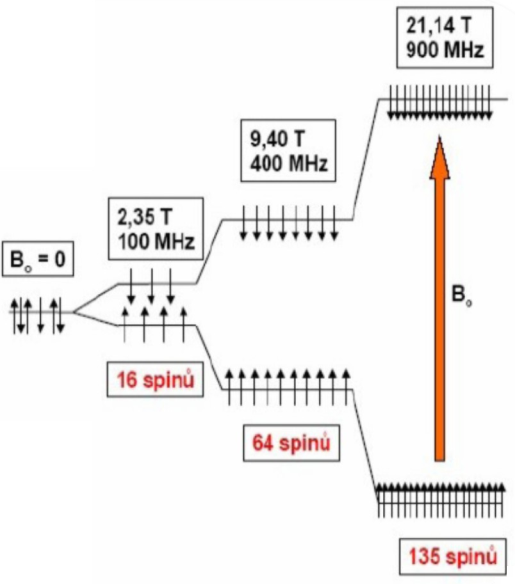
\includegraphics[height=.65\textheight]{img/NMR-levels.png}
		\caption*{Rozdělení spinů na hladinách v závislosti na síle magnetického pole}
	\end{figure}
	\vfill
}

\subsubsection{Radiofrekvenční pulsy}
\frame{
	\frametitle{}
	\vfill
	\begin{itemize}
		\item FT-NMR využívá k excitaci jaderných spinů radiofrekvenční pulsy.
		\item Ty excitují všechna měřená jádra, např. protony, najednou.
		\item Pulsy sklápí vektor magnetizace a způsobují jeho precesi.
		\item Délka pulsů se pohybuje v řádu $\mu$s.
		\item Čím je puls delší, tím je větší i sklápěcí úhel.
	\end{itemize}
	\begin{figure}
		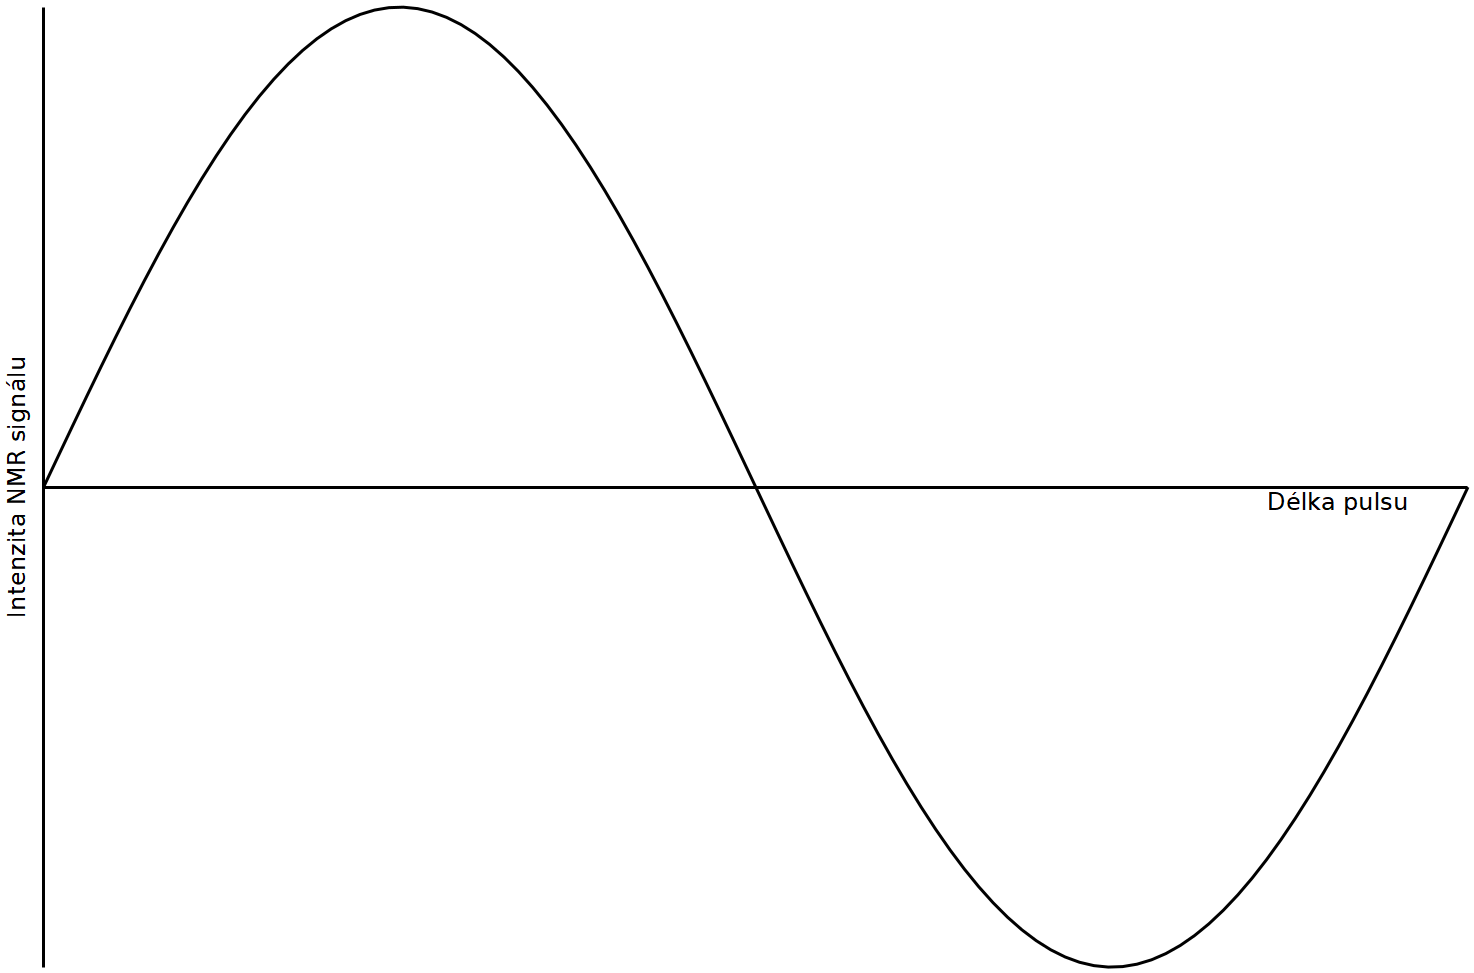
\includegraphics[width=.5\textwidth]{img/pulse/pulse-width.png}
	\end{figure}
	\vfill
}

\subsubsection{NMR magnety}
\frame{
	\frametitle{}
	\vfill
	\begin{itemize}
		\item Supravodivé magnety - nejběžnější v NMR
		\begin{itemize}
			\item Chlazené kapalným heliem (4--2,2 K)
			\item Magnetické pole až 28,2 T (1200 MHz)
		\end{itemize}
	\end{itemize}
	\begin{center}
		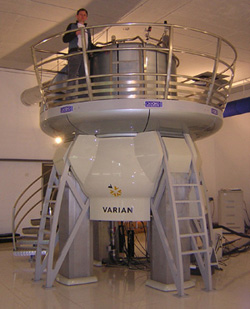
\includegraphics[keepaspectratio,width=5cm]{img/Varian-_900MHz_-_21.2_Tesla.jpg}
	\end{center}
	\vfill
}

\subsubsection{Závislost rezonanční frekvence na síle magnetického pole}
\frame{
	\frametitle{}
	\begin{tabular}{|l|l|l|}
		\hline
		$B_0$ [T] & $^1H$ [MHz] & $^{13}C$ [MHz] \\\hline
		1,41 & 60 & 15,1 \\\hline
		2,35 & 100 & 25,15 \\\hline
		7,05 & 300 & 75,4 \\\hline
		11,74 & 500 & 125,7 \\\hline
		14,09 & 600 & 150,9 \\\hline
		16,44 & 700 & 176,05 \\\hline
		19,97 & 850 & 213,78 \\\hline
		22,32 & 950 & 238,94 \\\hline
		28,2 & 1200 & 318,59 \\\hline
	\end{tabular}
	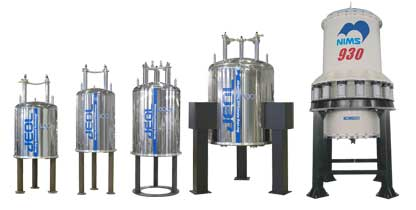
\includegraphics[keepaspectratio,width=5cm]{img/JEOL_NMR-Magnets_Family.jpg}
}

\subsubsection{NMR sondy}
\frame{
	\frametitle{}
	\vfill
	\textbf{NMR sondy}
	\begin{itemize}
		\item Hlavní funkcí je excitace spinového systému a snímání odezvy.
		\item Obsahují lockovací kanál.
		\item Udržují stabilní teplotu vzorku.
		\item Často obsahují také gradientovou cívku(y) pro experimenty využívající pulsní gradienty magnetického pole.
		\item Podle konstrukce se dělí:
		\begin{itemize}
			\item Teplé sondy
			\item Kryosondy
			\item Průtočné sondy
			\item Nanosondy
		\end{itemize}
	\end{itemize}
	\vfill
}

\frame{
	\frametitle{}
	\vfill
	\begin{figure}
		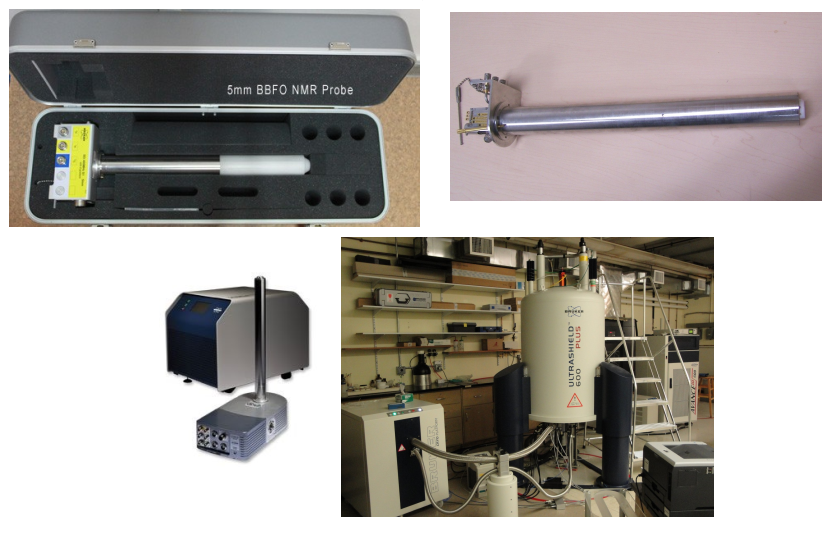
\includegraphics[height=.75\textheight]{img/NMR-probes.png}
		\caption*{Teplé sondy (nahoře) a kryosondy (dole)}
	\end{figure}
	\vfill
}

\subsubsection{Chemický posun}
\frame{
	\frametitle{}
	\vfill
	\begin{itemize}
		\item Izolovaná jádra stejného izotopu budou v magnetickém poli rezonovat při stejné frekvenci.
		\item Pokud uvažujeme molekuly, je každé jádro ovlivněno také lokálními magnetickými poli, které jsou generovány vazebnými elektrony. Tím dochází ke změně rezonanční frekvence daného jádra.
		\item Změna je dána tzv. chemickým okolím pozorovaného jádra a nazývá se \emph{chemický posun}. Označuje se $\delta$ a je dán vztahem:
	\end{itemize}
	\begin{center}
		$\delta = \frac{\nu - \nu_{TMS}}{\nu}$
	\end{center}
	\begin{itemize}
		\item $\nu_{TMS}$ je rezonanční frekvence standardu, $\nu$ je rezonanční frekvence signálu.
		\item Chemický posun je bezrozměrný, jelikož se jedná o velmi malé hodnoty, udává se v ppm.
		\item Chemický posun je, na rozdíl od rezonanční frekvence, nezávislý na hodnotě vnějšího magnetického pole.
	\end{itemize}
	\vfill
}

\frame{
	\frametitle{}
	\vfill
	\begin{figure}
		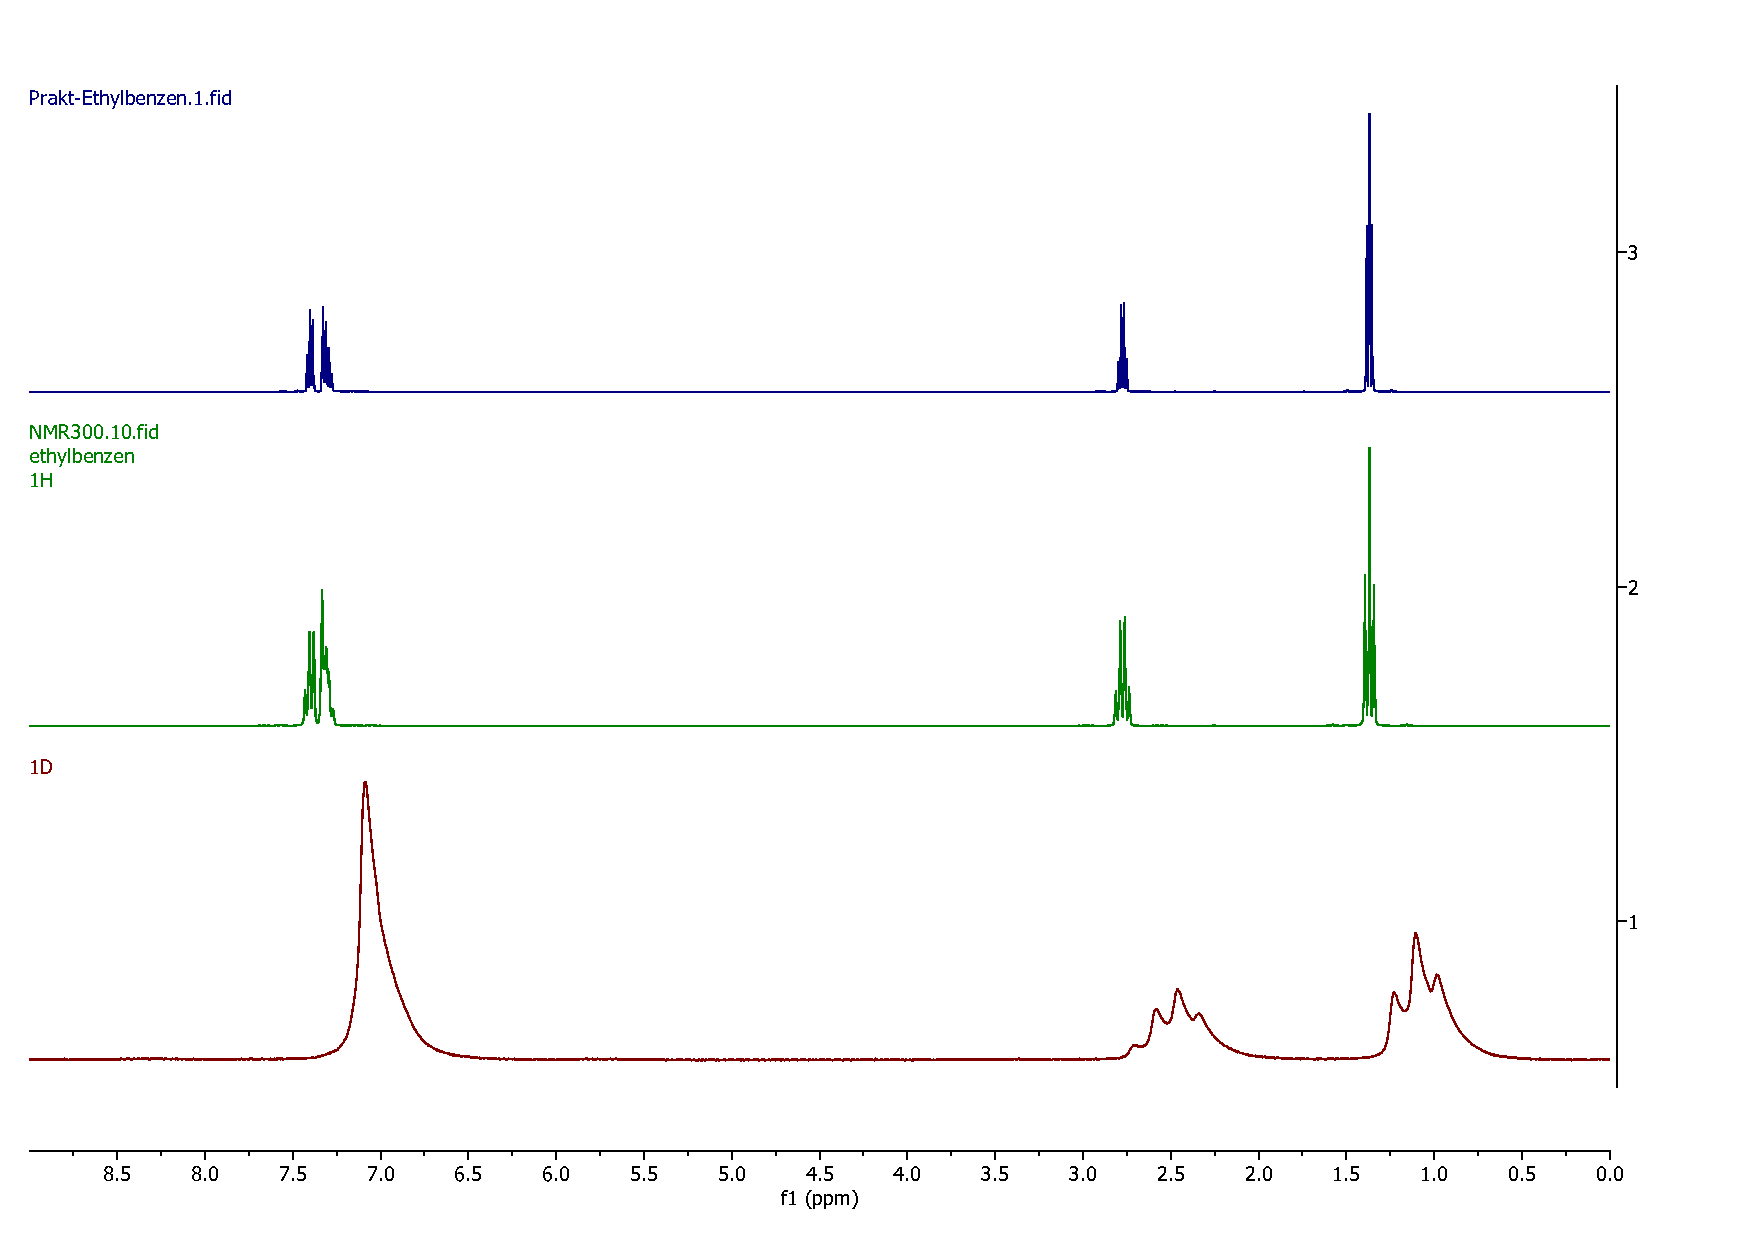
\includegraphics[height=.75\textheight]{img/Ethylbenzen-1H.pdf}
		\caption*{$^1$H NMR spektrum ethylbenzenu změření při 60, 300 a 500 MHz}
	\end{figure}
	\vfill
}

\subsubsection{Interakční konstanta}
\frame{
	\frametitle{}
	\vfill
	\begin{itemize}
		\item Pokud je v molekule více NMR aktivních jader, může docházet k jejich vzájemné interakci. Síla této interakce je dána hlavně počtem vazeb, které jádra oddělují.
		\item Velikost interakční konstanty je nezávislá na intenzitě magnetického pole.
	\end{itemize}
	\begin{center}
		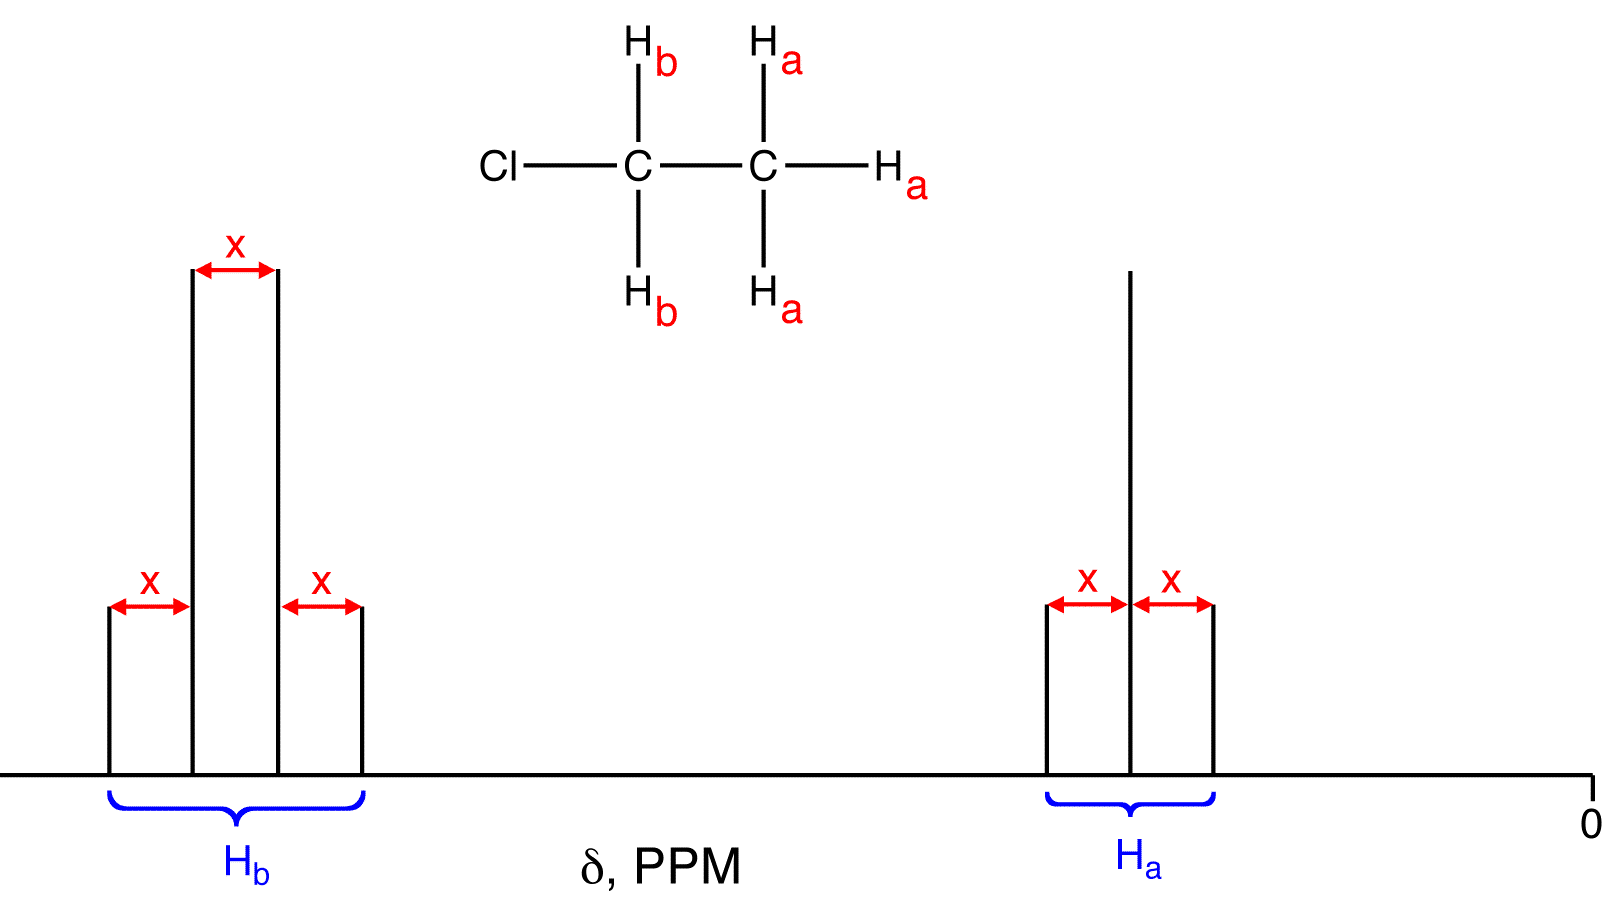
\includegraphics[keepaspectratio,width=9cm]{img/couplingconstant.png}
	\end{center}
	\vfill
}

\frame{
	\frametitle{}
	\vfill
	\begin{itemize}
		\item Způsob štěpení je dán počtem interagujících spinů.
		\item Pro jádra se spinem $\frac{1}{2}$ je velikost multipletu, tzn. počet signálů po štěpení a jejich vzájemná intenzita dána \textit{Pascalovým trojúhelníkem}.
	\end{itemize}
	\begin{tabular}{>{$n=}l<{$\hspace{6pt}}*{13}{c}}
		0 &&&&&&&1&&&&&&\\
		1 &&&&&&1&&1&&&&&\\
		2 &&&&&1&&2&&1&&&&\\
		3 &&&&1&&3&&3&&1&&&\\
		4 &&&1&&4&&6&&4&&1&&\\
		5 &&1&&5&&10&&10&&5&&1&\\
		6 &1&&6&&15&&20&&15&&6&&1
	\end{tabular}
	\vfill
}

\frame{
	\frametitle{}
	\vfill
	\begin{itemize}
		\item Pro jádra se spinem 1, např. $^2$H (D), musíme použít jinou variantu Pascalova trojúhelníku.
	\end{itemize}
	\begin{tabular}{>{$n=}l<{$\hspace{6pt}}*{11}{c}}
		0 &&&&&&1&&&&&\\
		1 &&&&&1&1&1&&&&\\
		2 &&&&1&2&3&2&1&&&\\
		3 &&&1&3&6&7&6&3&1&&\\
		4 &&1&4&10&16&19&16&10&4&1&\\
		5 &1&5&15&30&45&51&45&30&15&5&1 \\
	\end{tabular}

	\begin{figure}
		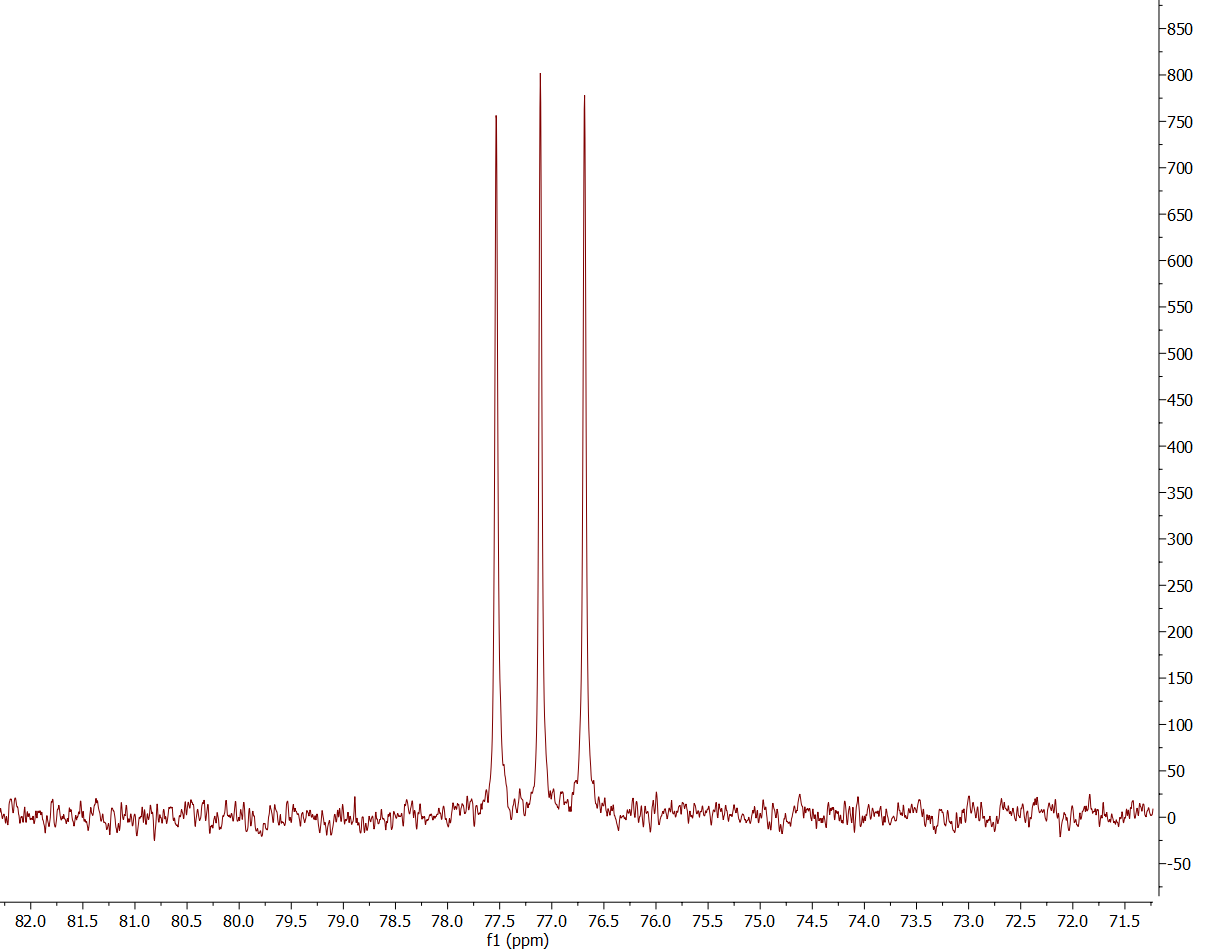
\includegraphics[height=.35\textheight]{img/CDCl3-13C-NMR.png}
		\caption*{$^{13}$C NMR \ce{CDCl3}, štěpení je způsobeno interakcí $^2$H-$^{13}$C}
	\end{figure}
	\vfill
}

\frame{
	\frametitle{}
	\vfill
	\begin{itemize}
		\item Velikost interakce se vyjadřuje pomocí interakční konstanty, která se označuje písmenem \textit{J}. Pro přesnější popis interakce se využívá
		indexů, např. interakci mezi atomy vodíku v~ethanolu (přes tři vazby H-C-C-H) vyjádříme $^3J_{HH}$. Její velikost se udává v Hz.
	\end{itemize}
	\begin{figure}
		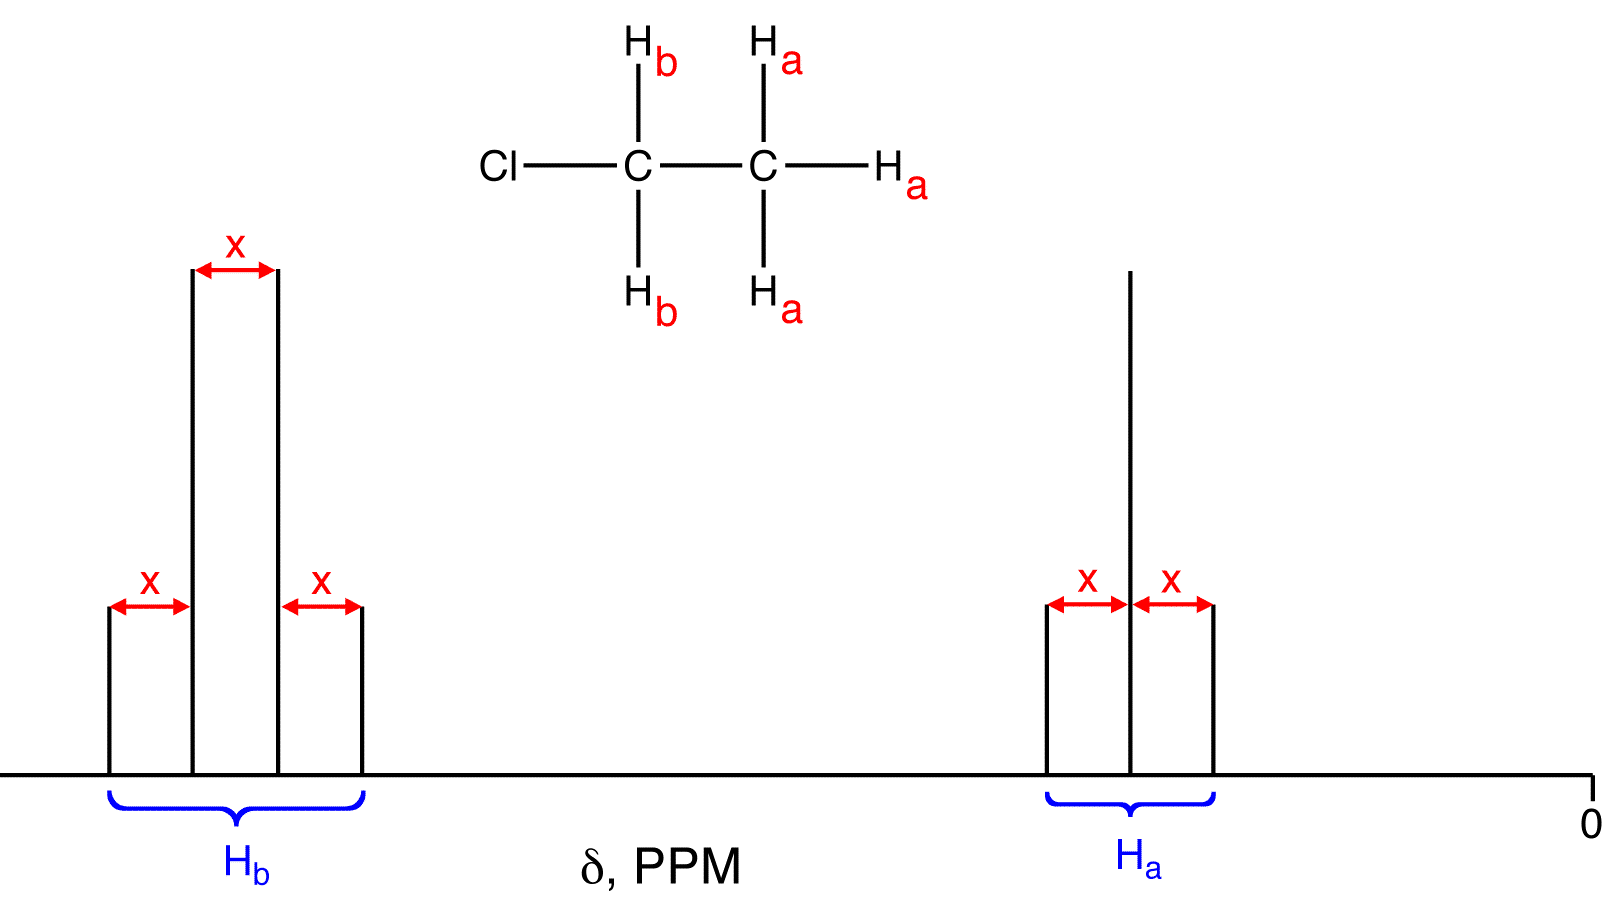
\includegraphics[keepaspectratio,width=10cm]{img/couplingconstant.png}
	\end{figure}
	\vfill
}

\subsubsection{Decoupling (dekaplink)}
\frame{
	\frametitle{}
	\begin{itemize}
		\item Štěpením signálů spektra je důležitou informací pro strukturní analýzu, zároveň ale zhoršuje poměr signál/šum.
		\item Pro potlačení štěpení se používá tzv. decoupling, kdy kontinuálně ozařujeme dekaplovaná jádra. Tím dojde k potlačení štěpení.
		\item Ztratíme ale informaci o kvantitativním složení vzorku, protože intenzita signálu v dekaplovaném spektru není úměrná koncentraci.
		\item Gated decoupling – neozařujeme během akvizice, nedojde k potlačení NOE.
		\item Inverse-gated decoupling – ozařujeme pouze během akvizice, vhodné pro jádra se záporným gyromagnetickým poměrem – $^{15}$N, $^{29}$Si.
	\end{itemize}
}

\subsubsection{2D NMR}
\frame{
	\frametitle{}
	\vfill
	\begin{itemize}
		\item Pro složitější molekuly už nemusí být 1D NMR spektrum čitelné.
		\item Rozlišení se dá zvýšit silnějším magnetickým polem.
		\item Lepší cestou je přechod na NMR experimenty ve dvou a více dimenzích.
		\item V dnešní době se rutinně využívá 2D a 3D NMR.
	\end{itemize}
	\begin{figure}
		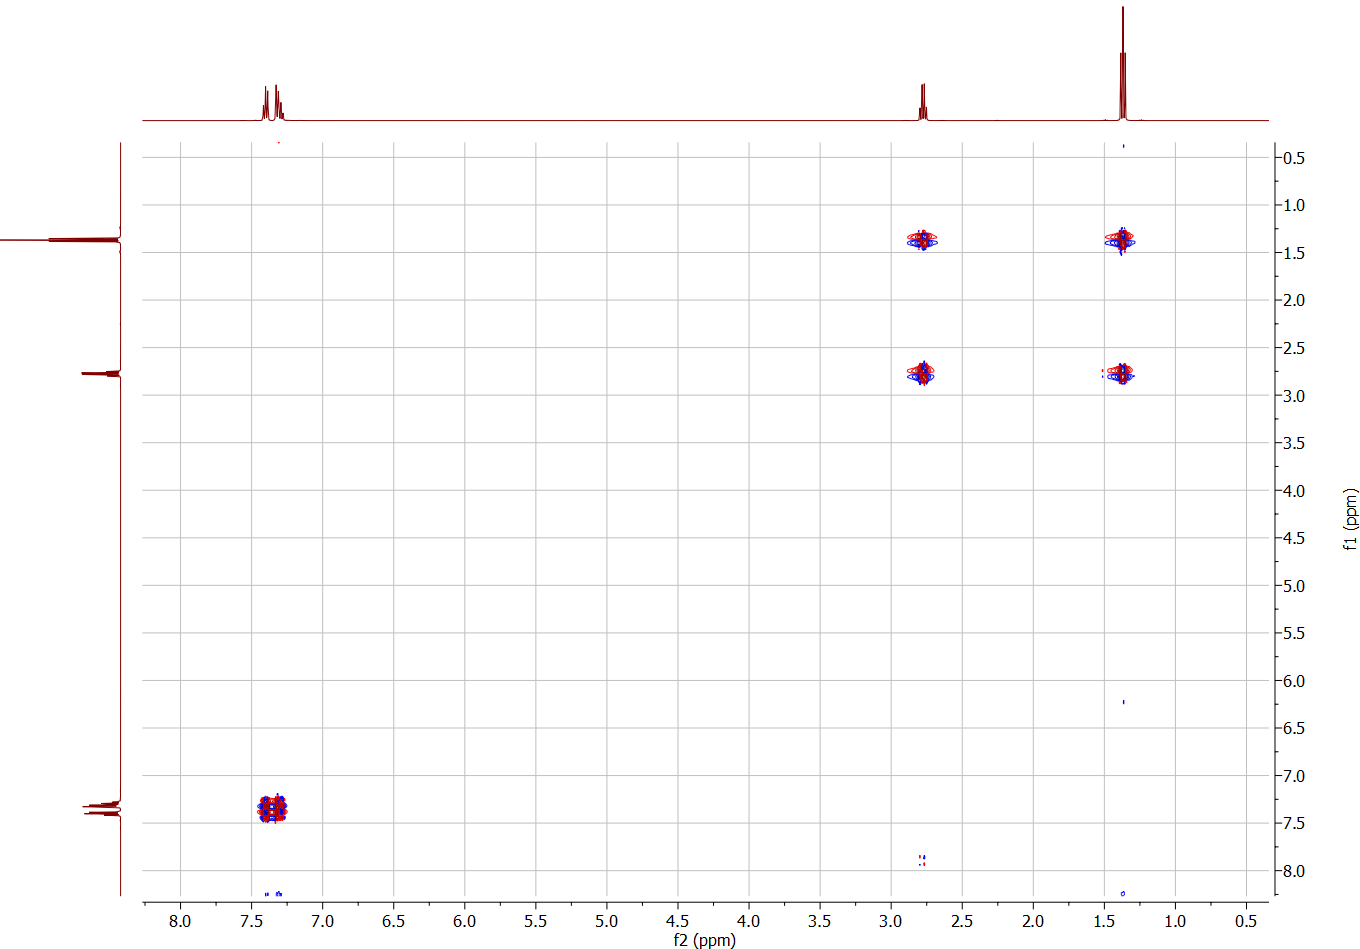
\includegraphics[height=.53\textheight]{img/Ethylbenzene-1H-COSY.png}
		\caption*{$^1$H-$^1$H COSY NMR}
	\end{figure}
	\vfill
}

\subsubsection{Vzorky pro NMR spektroskopii}
\frame{
	\frametitle{}
	\vfill
	\begin{columns}
		\begin{column}{0.7\textwidth}
			\begin{itemize}
				\item Využívají se tenkostěnné skleněné kyvety, které se umisťují do plastových nebo keramických rotorků. Průměr kyvet je nejčastěji 3, 5 nebo 10 mm.
				\item Pro měření je nutné připravit roztok měřené látky v~deuterovaném rozpouštědle. Signál $^2$H~(D) se používá k~lockování vzorku.
				\item Vzorky reakčních směsí se často měří v~koaxiálním uspořádání, kdy se kyveta se vzorkem vloží do kyvety s deuterovaným
				rozpouštědlem.
				\item Signál deuterovaného rozpouštědla lze využít i~jako standard ke kalibraci spektra.
			\end{itemize}
		\end{column}
		\begin{column}{0.3\textwidth}
			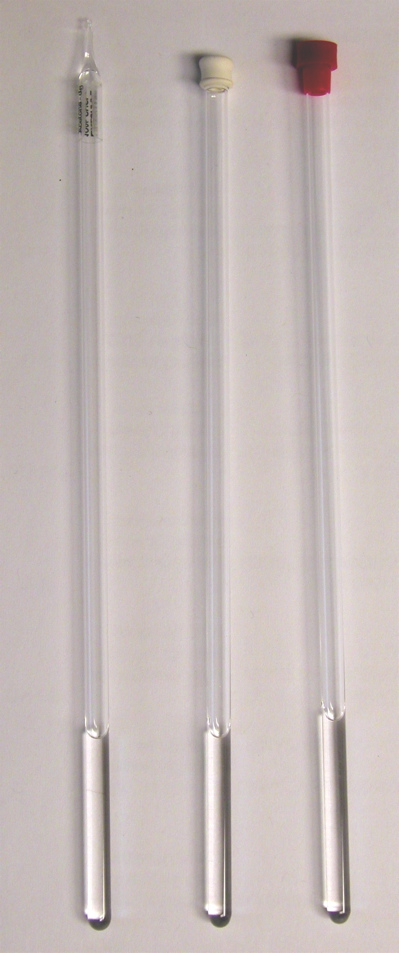
\includegraphics[keepaspectratio,width=3cm]{img/NMR-tubes.jpg}
		\end{column}
	\end{columns}
	\vfill
}

\subsubsection{NMR v pevné fázi}
\frame{
	\frametitle{}
	\vfill
	\begin{itemize}
		\item MAS NMR - Magic Angle Spinning.
		\item Vzorek je napěchován do keramického rotoru a rotuje pod úhlem 54,7$^{\circ}$ ($\cos^2\theta_m=\frac{1}{3}$, magický úhel).
		\item Rotace při rychlostech 0-130 kHz.
		\item Pro měření málo citlivých jader se využívá cross-polarizace.
	\end{itemize}
	\begin{figure}
		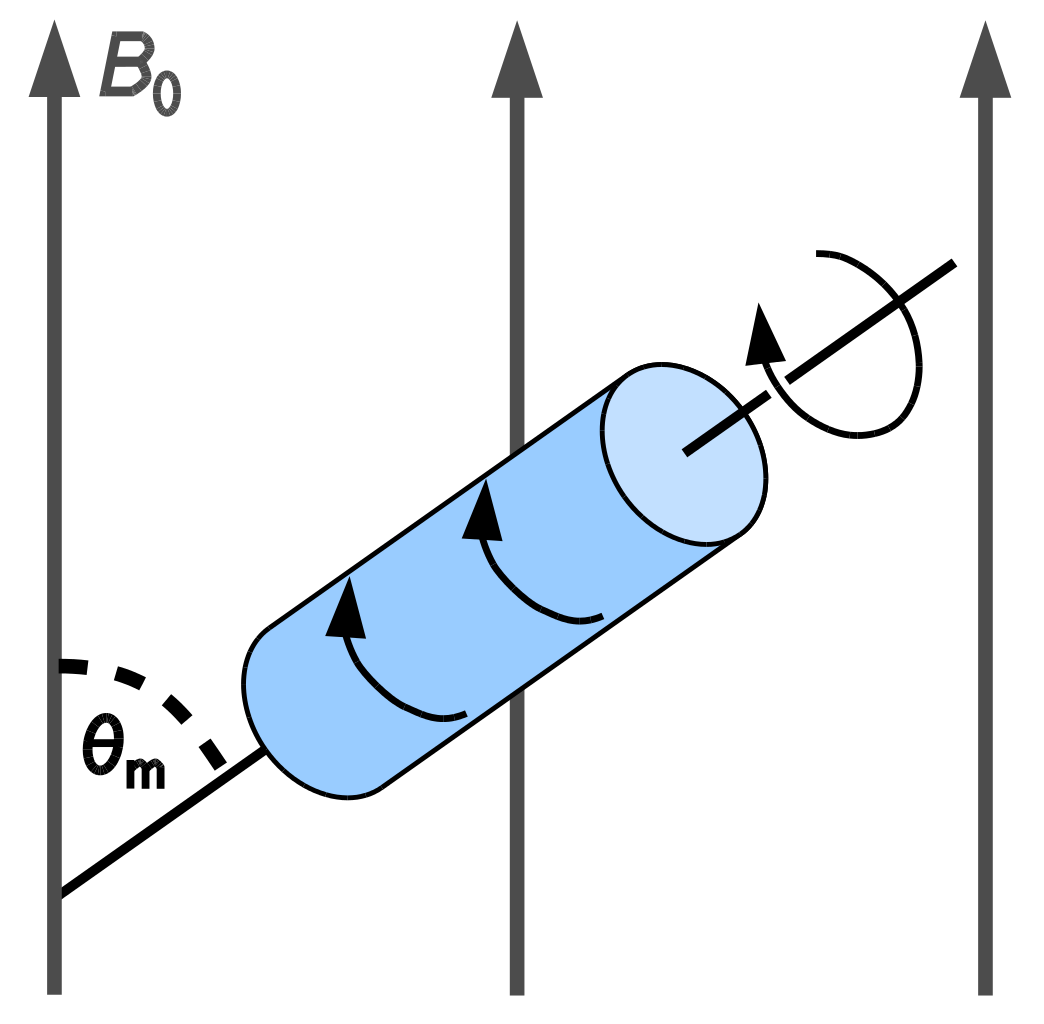
\includegraphics[height=.45\textheight]{img/NMR-MAS-angle.png}
		\caption*{Magický úhel.\footnote[frame]{Zdroj: \href{https://commons.wikimedia.org/wiki/File:MagicAngleSpinning.svg}{Dtrx/Commons}}}
	\end{figure}
	\vfill
}

\frame{
	\frametitle{}
	\vfill
	\begin{figure}
		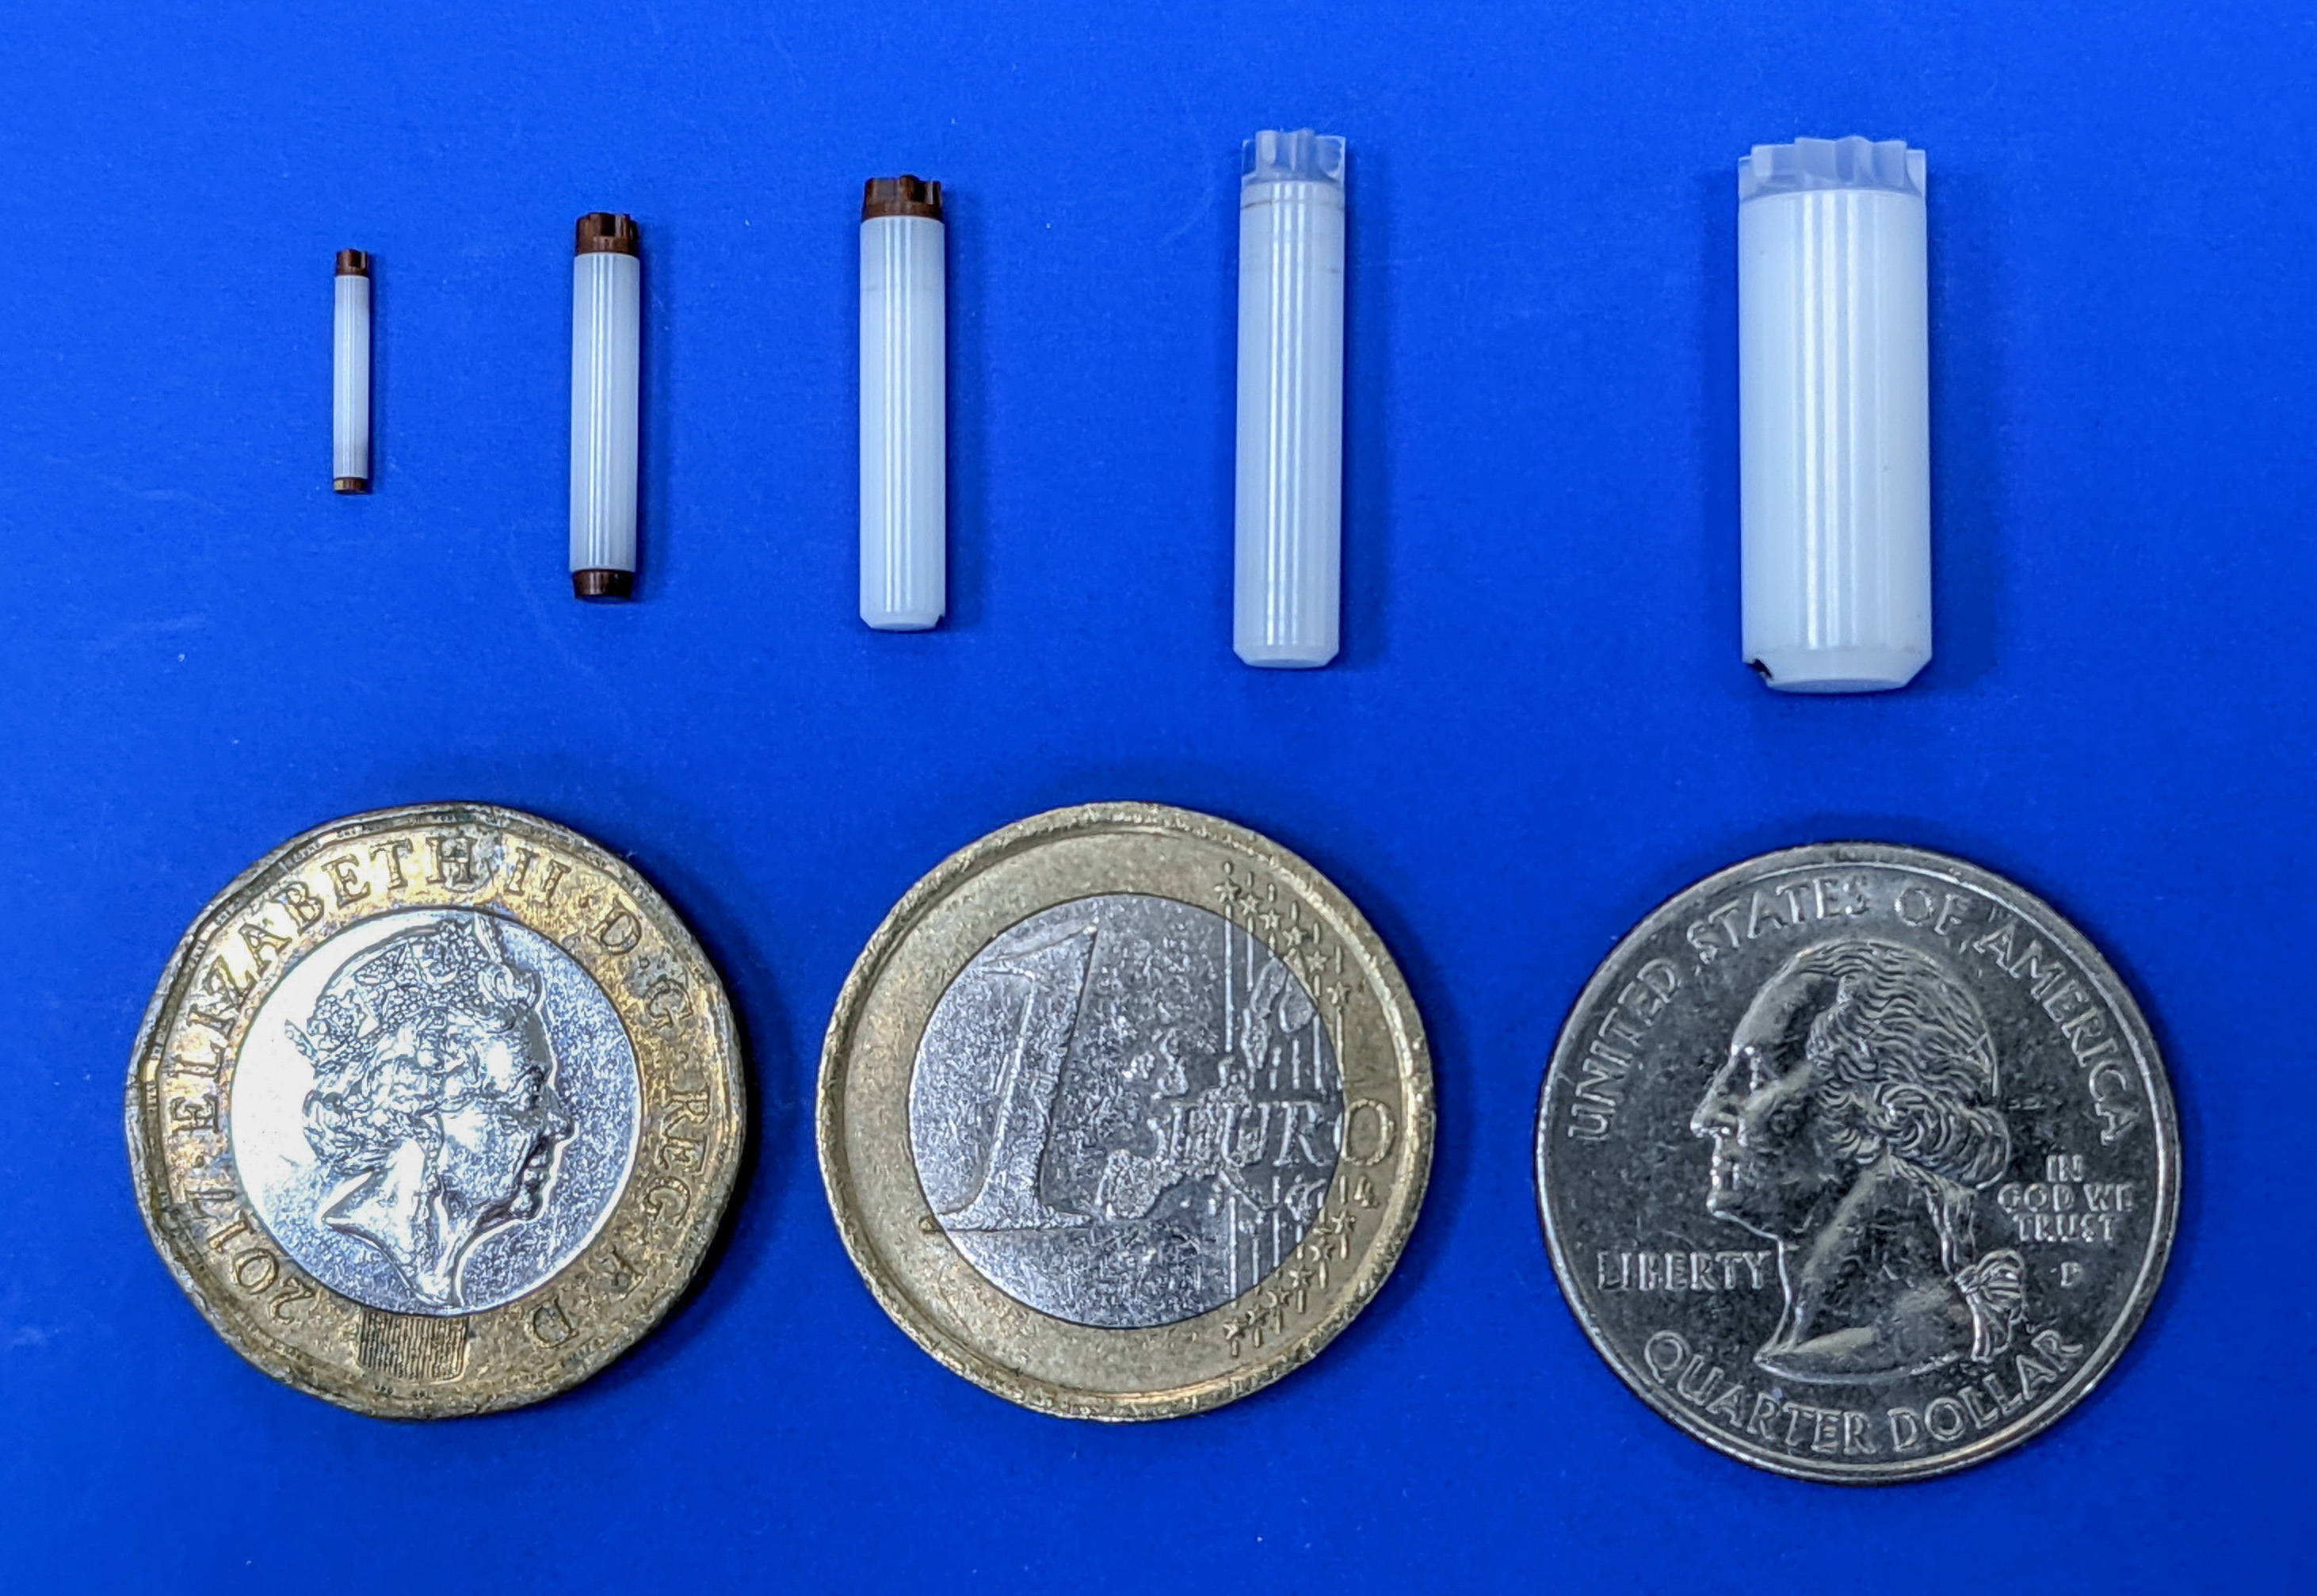
\includegraphics[height=.68\textheight]{img/NMR-MAS-rotors.jpg}
		\caption*{Rotorky pro MAS NMR.\footnote[frame]{Zdroj: \href{https://commons.wikimedia.org/wiki/File:MAS_rotors.jpg}{Thomas Kress/Commons}}}
	\end{figure}
	\vfill
}

\subsection{Povrchová analýza}
\frame{
	\frametitle{}
	\vfill
	\begin{columns}
		\begin{column}{.6\textwidth}
			\textbf{Povrchová analýza}
			\begin{itemize}
				\item Skupina metod pro stanovení měrného povrchu a porosity materiálů.
				\item \textbf{Měrný povrch} - povrch materiálu vztažený na jednotku hmotnosti.
				\item \textbf{Rtuťová intruzní porozimetrie} -- založena na vtlačování rtuti do pórů. Používá se pro stanovení pórů o velikostech od 4~nm do stovek mikrometrů.
				\item \textbf{Plynová porozimetrie} -- sorpce plynu na povrch vzorku. Používá se pro stanovení pórů o velikostech od 0,33~nm do stovek nanometrů.
			\end{itemize}
		\end{column}
		\begin{column}{.5\textwidth}
			\begin{center}
				\adjincludegraphics[width=.9\textwidth]{img/ZIF-8.png}
			\end{center}
		\end{column}
	\end{columns}
	\vfill
}

\frame{
	\frametitle{}
	\vfill
	Měrný povrch je důležitou charakteristikou katalyzátorů, sorpčních materiálů, apod.
	\begin{columns}
		\begin{column}{.5\textwidth}
			\begin{tabular}{|l|l|}
				\hline
				\textbf{Materiál} & \textbf{SA [m$^2$.g$^{-1}$]} \\\hline
				MOF & 7140 \\\hline
				Grafen & 2700 \\\hline
				Aktivní uhlí & 500--3000 \\\hline
				MCM-41 (\ce{SiO2}) & 1000 \\\hline
				Molekulová síta & až 1000 \\\hline
				Faujesite & 900 \\\hline
				Alumina & 200 \\\hline
				\ce{CaCO3} & 3 \\\hline
			\end{tabular}

		\end{column}
		\begin{column}{.5\textwidth}
			\begin{center}
				\adjincludegraphics[width=.8\textwidth]{img/Radial_mesoporous_silica.jpg}

				\textbf{Velikost pórů:}

				\begin{tabular}{ll}
					Mikropóry & $<$2 nm \\
					Mezopóry & 2--50 nm \\
					Makropóry & $>$50 nm \\
				\end{tabular}
			\end{center}
		\end{column}
	\end{columns}
	\vfill
}

\subsection{Rtuťová porozimetrie}
\frame{
	\frametitle{}
	\vfill
	\begin{columns}
		\begin{column}{.6\textwidth}
			\begin{itemize}
				\item Do vzorku je vtláčena rtuť.
				\item Jde o destruktivní metodu.
				\item Velikost pórů od 4~nm do stovek mikrometrů.
				\item Čím vyšší tlak působí, tím se dostává rtuť do menších pórů, spodní hranici ovlivňuje maximální možný tlak.
				\item Měření je poměrně rychlé.
				\item Problémem je toxicita rtuti.
			\end{itemize}
		\end{column}
		\begin{column}{.5\textwidth}
			\begin{center}
				\adjincludegraphics[width=.9\textwidth]{img/Hg-porosimeter.png}
			\end{center}
		\end{column}
	\end{columns}
	\vfill
}

\frame{
	\frametitle{}
	\vfill
	\adjincludegraphics[width=\textwidth]{img/Hg-porosimetry.png}
	\vfill
}

\subsection{Plynová porozimetrie}
\frame{
	\frametitle{}
	\vfill
	\begin{itemize}
		\item Brunauer–Emmett–Teller (BET) -- velmi používaný způsob výpočtu měrného povrchu.
		\item Využívá začátek adsorpční izotermy (P/P$_0$ 0-0,3), kdy lze předpokládat vznik monovrstvy.
		\item Vychází z několika (bohužel nereálných) předpokladů:
		\begin{itemize}
			\item plochý povrch adsorbentu
			\item všechna adsorpční místa jsou energeticky ekvivalentní (homogenní)
			\item neexistují vzájemné interakce mezi adsorbovanými molekulami
			\item adsorpční energie je pro všechny molekuly vyjma první vrstvy rovna energii zkapalnění
			adsorbátu
			\item neomezený počet adsorpčních vrstev, nekonečný při nasyceném tlaku
			\item rychlost desorpce molekul v určité vrstvě je rovna rychlosti kondenzace ve vrstvě o jednu níže
		\end{itemize}
		\item $\frac{\frac{p}{p_0}}{V(1-\frac{p}{p_0})} = \frac{1}{CV_m} + \frac{C-1}{CV_m}\frac{p}{p_0}$
	\end{itemize}
	\vfill
}

\frame{
	\frametitle{}
	\vfill
	\begin{itemize}
		\item Dříve se pro stanovení BET povrchu využívala sorpce v dusíku, dnes se doporučuje argon.
		\item Molekula dusíku může zkreslovat výslednou hodnotu kvůli kvadrupolárnímu momentu molekuly dusíku. Může docházet k interakci s polárními místy na povrchu vzorku.
		\item Pro měření s argonem potřebujeme kapalný argon nebo zařízení, které dokáže temperovat kyvetu na teplotu kapalného argonu.
	\end{itemize}
	\begin{columns}
		\begin{column}{.5\textwidth}
			\adjincludegraphics[height=.4\textheight]{img/Cryosync2.png}
		\end{column}
		\begin{column}{.5\textwidth}
			\adjincludegraphics[height=.4\textheight]{img/Cryosync1.png}
		\end{column}
	\end{columns}
	\vfill
}

\frame{
	\frametitle{}
	\vfill
	\begin{figure}
		\adjincludegraphics[width=.9\textwidth]{img/BET.png}
		\caption*{Jedenáctibodová izoterma}
	\end{figure}
	\vfill
}

\frame{
	\frametitle{}
	\vfill
	\begin{figure}
		\adjincludegraphics[width=.9\textwidth]{img/BET2.png}
		\caption*{Jedenáctibodová BET křivka}
	\end{figure}
	\vfill
}

\subsection{Termická analýza}
\frame{
	\frametitle{}
	\vfill
	\begin{itemize}
		\item Soubor metod sledujících chování vzorku během definovaného teplotního programu
		\item TG - termogravimetrie - sledujeme změny hmotnosti vzorku
		\item DTA - diferenční termická analýza - sledujeme rozdíl teplot mezi vzorkem a referencí během teplotního programu
		\item DSC - diferenční skenovací kalorimetrie - měříme tepelný tok mezi vzorkem a referencí
		\item STA - simultánní termická analýza
		\item TMA - Termomechanická analýza - sledujeme deformace zatíženého vzorku během teplotního programu
	\end{itemize}
	\vfill
}

\subsubsection{Termogravimetrie}
\frame{
	\frametitle{}
	\vfill
	\begin{itemize}
		\item Měříme změny hmotnosti vzorku při jeho plynulém ohřevu nebo ochlazování
		\item Změny hmotnosti se vyjadřují jako závislost na teplotě nebo čase analýzy
		\item  Během ohřevu může docházet k poklesu hmotnosti vzorku, z~důvodu uvolňování plynu, např. vody nebo oxidu uhličitého
		\item Může také docházet ke zvyšování hmotnosti vzorku reakcí s~atmosférou - oxidace vzorku
		\item TG křivky podávají informace o složení zkoumaného vzorku, jeho tepelné stálosti, teplotním rozkladu a také o produktech vznikajících při rozkladu
		\item TG křivka ve svém průběhu obsahuje úseky vodorovné s osou x, tzv. prodlevy, a~zlomy. Prodlevy jsou úseky, kdy ještě nedošlo k žádné změně hmotnosti vzorku. Zlomy naopak naznačují, že se analyzovaný vzorek začíná rozkládat (mění svoji hmotnost)
	\end{itemize}
	\vfill
}

\frame{
	\frametitle{}
	\vfill
	\begin{figure}
		\adjincludegraphics[width=.9\textwidth]{img/tg-skalice.png}
		\caption*{TG křivka modré skalice}
	\end{figure}
	\vfill
}

\subsubsection{DTA}
\frame{
	\frametitle{}
	\begin{columns}
		\begin{column}{0.5\textwidth}
			\vfill
			\begin{itemize}
				\item Diferenční Termická Analýza
				\item Předchůdce DSC, jednodušší instrumentace
				\item Umožňuje měřit tepelné změny vzorku během analýzy
				\item Měříme rozdíl teploty kelímku se vzorkem a referenčního kelímku
			\end{itemize}
			\vfill
		\end{column}
		\begin{column}{0.5\textwidth}
			\adjincludegraphics[width=\textwidth]{img/DTA.jpg}
		\end{column}
	\end{columns}
}

\frame{
	\frametitle{}
	\vfill
	\begin{columns}
		\begin{column}{0.8\textwidth}
			\begin{itemize}
				\item Pro redukční prostředí se využívá TG/DTA držák s termočlánky typu W.
				\item Velmi citlivý na stopy kyslíku - nutno používat Zr getter.
				\item Umožňuje měření v redukční atmosféře, např. ve formovacím plynu (H$_2$/N$_2$ 5:95).
				\item Redukce oxidů thoria, uranu.
			\end{itemize}
		\end{column}
		\begin{column}{0.2\textwidth}
			\adjincludegraphics[width=\textwidth]{img/Zr-getter.png}
		\end{column}
	\end{columns}
	\vfill
}

\frame{
	\frametitle{}
	\vfill
	\adjincludegraphics[height=.95\textheight]{img/DTA-W.jpg}
	\vfill
}

\subsubsection{DSC}
\frame{
	\frametitle{}
	\vfill
	\begin{itemize}
		\item DSC s kompenzací příkonu - podstatou DSC s kompenzací příkonu je zachování nulového teplotního rozdílu mezi měřeným a srovnávacím vzorkem. Tato varianta DSC je charakterizována dvěma oddělenými měřícími celami a dvěma tepelnými zdroji a měříme tedy elektrický příkon, který je potřebný k udržení konstantní teploty obou vzorků.
		\item DSC s tepelným tokem - druhou variantou je metoda DSC s tepelným tokem. Měření rozdílu příkonu je nahrazeno měřením rozdílu teplot vzorku a srovnávacího vzorku, které jsou umístěny ve společné peci a jsou spojeny tepelným mostem. Se znalostí tepelného odporu mezi pecí a vzorkem a referencí lze považovat tepelný tok od vzorku nebo ke vzorku za úměrný rozdílu teplot. Teplota vzorku je měřena termočlánkem, který je v kontaktu se vzorkem.
	\end{itemize}
	\vfill
}

\frame{
	\frametitle{}
	\vfill
	\adjincludegraphics[width=\textwidth]{img/Power-compensation-DSC.png}
	\vfill
}

\frame{
	\frametitle{}
	\vfill
	\begin{figure}
		\adjincludegraphics[height=.8\textheight]{img/STA449C-drzak2.jpg}

	\end{figure}
	\vfill
}

\frame{
	\frametitle{}
	\vfill
	\begin{figure}
		\adjincludegraphics[width=\textwidth]{img/dsc-skalice.png}
		\caption*{DSC křivka modré skalice}
	\end{figure}
	\vfill
}

\subsubsection{STA}
\frame{
	\frametitle{}
	\vfill
	\begin{itemize}
		\item Simultánní metody (STA) – umožňují sledovat více fyzikálních vlastností během jednoho měření. Výhodou tohoto přístupu je, že nemusíme připravovat nové vzorky a máme tak dány stejné experimentální podmínky. Na druhou stranu ale tyto podmínky musí vyhovovat všem použitým metodám.
		\item Mezi nejvíce rozšířenou dvojici metod patří TG-DTA a~TG-DSC. Tyto metody se totiž dobře doplňují.
	\end{itemize}
	\vfill
}

\frame{
	\frametitle{}
	\vfill
	\begin{figure}
		\adjincludegraphics[width=\textwidth]{img/tg-dsc-skalice.png}
		\caption*{STA modré skalice}
	\end{figure}
	\vfill
}

\subsubsection{Coupling TGA/IR}
\frame{
	\frametitle{}
	\vfill
	\begin{itemize}
		\item Plyny vznikající během degradace vzorku vedeme do měřící cely a pomocí IR spektroskopie stanovíme jejich složení
		\item Během transportu plynů z pece do měřící cely dochází k velkému zředění plynu, proto je nutné používat citlivější detektory (MCT)
	\end{itemize}
	\adjincludegraphics[width=10cm,valign=l]{img/tg-irFoto.jpg}
	\vfill
}

\frame{
	\frametitle{}
	\vfill
	\adjincludegraphics[height=.8\textheight]{img/tg-ir.png}
	\vfill
}

\frame{
	\frametitle{}
	\vfill
	\adjincludegraphics[height=.9\textheight]{img/csm_Perseus_STA_449_F1_Jupiter_Bruker_Alpha_80a815b103.png}
	\vfill
}

\subsection{Mikroskopie}
\frame{
	\frametitle{}
	\vfill
	\begin{itemize}
		\item Pro analýzu prášků a povrchových vrstev se využívá \textit{elektronová mikroskopie}.
		\item Místo světla využívá proud urychlených elektronů, což umožňuje zlepšit rozlišení fotografie.
		\item Získané obrázky jsou černobílé, ale je možné je kolorovat na základě dalších dat, např. prvkového složení.
		\item Druhy elektronové mikroskopie:
		\begin{itemize}
			\item SEM -- skenovací elektronová mikroskopie
			\item TEM -- transmisní elektronová mikroskopie
			\item AFM -- mikroskopie atomárních sil
		\end{itemize}
		\item EDX -- energiově dispezní RTG spektroskopie (Energy-dispersive \mbox{X-ray} spectroscopy). Analytická technika poskytující prvkové složení vzorku.
		\item Snímání objektu probíhá zpravidla ve vakuu a vzorky by měly být vodivé.
	\end{itemize}
	\vfill
}

\frame{
	\frametitle{}
	\vfill
	\begin{columns}
		\begin{column}{.7\textwidth}
			\begin{figure}
				\adjincludegraphics[width=\textwidth]{img/Schema_MEB.png}
				\caption*{Schéma SEM.\footnote[frame]{Zdroj: \href{https://commons.wikimedia.org/wiki/File:Schema_MEB_(en).svg}{Steff/Commons}}}
			\end{figure}
		\end{column}
		\begin{column}{.3\textwidth}
			\begin{figure}
				\adjincludegraphics[width=1.3\textwidth]{img/Electron_emission.png}
				\caption*{Emise elektronů.\footnote[frame]{Zdroj: \href{https://commons.wikimedia.org/wiki/File:Electron_emission_mechanisms.svg}{Rob Hurt/Commons}}}
			\end{figure}
		\end{column}
	\end{columns}
	\vfill
}

\frame{
	\frametitle{}
	\vfill
	\begin{figure}
		\adjincludegraphics[height=.67\textheight]{img/Germanium_Telluride_nanowires.jpg}
		\caption*{Nanovlákna GeTe.\footnote[frame]{Zdroj: \href{https://commons.wikimedia.org/wiki/File:Germanium_Telluride_nanowires.jpg}{Fionán/Commons}}}
	\end{figure}
	\vfill
}

\frame{
	\frametitle{}
	\vfill
	\begin{figure}
		\adjincludegraphics[height=.67\textheight]{img/Quasimodopsis_riedeli_SEM.jpg}
		\caption*{SEM snímek \textit{Quasimodopsis riedeli}.\footnote[frame]{Zdroj: \href{https://commons.wikimedia.org/wiki/File:Quasimodopsis_riedeli_SEM.jpg}{Michael S. Caterino/Commons}}}
	\end{figure}
	\vfill
}

\frame{
	\frametitle{}
	\vfill
	\begin{figure}
		\adjincludegraphics[height=.67\textheight]{img/EDS_-_Rimicaris_exoculata.png}
		\caption*{Ukázka EDX spektra.\footnote[frame]{Zdroj: \href{https://commons.wikimedia.org/wiki/File:EDS_-_Rimicaris_exoculata.png}{Hat'nCoat/Commons}}}
	\end{figure}
	\vfill
}

\frame{
	\frametitle{}
	\vfill
	\begin{columns}
		\begin{column}{.7\textwidth}
			\begin{figure}
				\adjincludegraphics[height=.63\textheight]{img/TEM_philips_EM_430.jpg}
				\caption*{TEM mikroskop.\footnote[frame]{Zdroj: \href{https://commons.wikimedia.org/wiki/File:TEM_philips_EM_430.jpg}{KristianMolhave/Commons}}}
			\end{figure}
		\end{column}
		\begin{column}{.3\textwidth}
			\begin{figure}
				\adjincludegraphics[height=.63\textheight]{img/Electron_microscope.png}
				\caption*{Schéma TEM mikroskopu.\footnote[frame]{Zdroj: \href{https://commons.wikimedia.org/wiki/File:Electron_microscope.svg}{Superborsuk/Commons}}}
			\end{figure}
		\end{column}
	\end{columns}
	\vfill
}

\frame{
	\frametitle{}
	\vfill
	\begin{figure}
		\adjincludegraphics[height=.65\textheight]{img/TEM_images_of_silica.jpg}
		\caption*{TEM snímek hybridní siliky.\footnote[frame]{Zdroj: \href{https://commons.wikimedia.org/wiki/File:TEM_images_of_silica-organic_matrix-based_suspension.jpg}{Florentyna/Commons}}}
	\end{figure}
	\vfill
}

\frame{
	\frametitle{}
	\vfill
	\begin{figure}
		\adjincludegraphics[height=.67\textheight]{img/AFMsetup.jpg}
		\caption*{Schéma AFM.\footnote[frame]{Zdroj: \href{https://commons.wikimedia.org/wiki/File:AFMsetup.jpg}{KristianMolhave/Commons}}}
	\end{figure}
	\vfill
}

\frame{
	\frametitle{}
	\vfill
	\begin{figure}
		\adjincludegraphics[height=.67\textheight]{img/AFM_-_detail.jpg}
		\caption*{AFM mikroskop.\footnote[frame]{Zdroj: \href{https://commons.wikimedia.org/wiki/File:AFM_-_detail.jpg}{Laundry/Commons}}}
	\end{figure}
	\vfill
}

\frame{
	\frametitle{}
	\vfill
	\begin{figure}
		\adjincludegraphics[height=.67\textheight]{img/AFM_3D_Topography.jpg}
		\caption*{AFM snímek nanočástic palladia.\footnote[frame]{Zdroj: \href{https://commons.wikimedia.org/wiki/File:AFM_3D_Topography_Image_of_Palladium_Nanoparticles_on_Chitosan_Film.tif}{Mehrabanian/Commons}}}
	\end{figure}
	\vfill
}

\subsection{Dynamický rozptyl světla -- DLS}
\frame{
	\frametitle{}
	\vfill
	\begin{itemize}
		\item DLS je metoda určená pro měření velikosti částic v submikronové oblasti.\footnote[frame]{\href{http://www.chemicke-listy.cz/ojs3/index.php/chemicke-listy/article/view/506}{Dynamický rozptyl světla v analýze koloidních systémů}}
		\item Principem je měření fluktuace intenzity světla z laserového zdroje.
		\item Tyto fluktuace jsou způsobeny interferenčním zeslabovaním a zesilováním světla rozptýleného na pohybujících se částicích v disperzním systému.
		\item Tyto částice podléhají Brownovu pohybu\footnote[frame]{Náhodný pohyb mikroskopických částic v plynném nebo kapalném prostředí}, čím je částice menší, tím se pohybuje rychleji a tím rychleji dochází ke změně intenzity rozptýleného záření.
	\end{itemize}
	\vfill
}

\frame{
	\frametitle{}
	\vfill
	\begin{figure}
		\adjincludegraphics[height=.7\textheight]{img/DLS.png}
		\caption*{Princip DLS.\footnote[frame]{Zdroj: \href{https://commons.wikimedia.org/wiki/File:DLS.svg}{Mike Jones/Commons}}}
	\end{figure}
	\vfill
}

\input{../Last}

\end{document}